%%
%% This is file `sigconf.tex',
%% generated with the docstrip utility.
%%
%% The original source files were:
%%
%% samples.dtx  (with options: `all,proceedings,sigconf')
%% 
%% IMPORTANT NOTICE:
%% 
%% For the copyright see the source file.
%% 
%% Any modified versions of this file must be renamed
%% with new filenames distinct from sigconf.tex.
%% 
%% For distribution of the original source see the terms
%% for copying and modification in the file samples.dtx.
%% 
%% This generated file may be distributed as long as the
%% original source files, as listed above, are part of the
%% same distribution. (The sources need not necessarily be
%% in the same archive or directory.)
%%
%%
%% Commands for TeXCount
%TC:macro \cite [option:text,text]
%TC:macro \citep [option:text,text]
%TC:macro \citet [option:text,text]
%TC:envir table 0 1
%TC:envir table* 0 1
%TC:envir tabular [ignore] word
%TC:envir displaymath 0 word
%TC:envir math 0 word
%TC:envir comment 0 0
%%
%% The first command in your LaTeX source must be the \documentclass
%% command.
%%
%% For submission and review of your manuscript please change the
%% command to \documentclass[manuscript, screen, review]{acmart}.
%%
%% When submitting camera ready or to TAPS, please change the command
%% to \documentclass[sigconf]{acmart} or whichever template is required
%% for your publication.
%%
%%
% \documentclass[sigconf]{acmart}
\documentclass[sigconf,review]{acmart}
\usepackage{subcaption}
\usepackage{xcolor}

\makeatletter
\renewcommand{\today}{}
\makeatother

\usepackage{amsmath}
\DeclareMathOperator*{\argmax}{arg\,max}
\newcommand{\abs}[1]{\left| #1 \right|}

\usepackage{algorithm}
\usepackage{algpseudocode}


\newcommand{\ys}[1]{\textcolor{red}{[YS: #1]}}
\newcommand{\td}[1]{\textcolor{blue}{[TODO: #1]}}

%%
%% \BibTeX command to typeset BibTeX logo in the docs
\AtBeginDocument{%
  \providecommand\BibTeX{{%
    Bib\TeX}}}

%% Rights management information.  This information is sent to you
%% when you complete the rights form.  These commands have SAMPLE
%% values in them; it is your responsibility as an author to replace
%% the commands and values with those provided to you when you
%% complete the rights form.
\setcopyright{acmlicensed}
\copyrightyear{2018}
\acmYear{2018}
\acmDOI{XXXXXXX.XXXXXXX}
%% These commands are for a PROCEEDINGS abstract or paper.
\acmConference[ACM KDD '27]{Proceedings of the 33rd ACM SIGKDD Conference on Knowledge Discovery and Data Mining}{August 01--05,
  2027}{San Jose, CA}
%%
%%  Uncomment \acmBooktitle if the title of the proceedings is different
%%  from ``Proceedings of ...''!
%%
%%\acmBooktitle{Woodstock '18: ACM Symposium on Neural Gaze Detection,
%%  June 03--05, 2018, Woodstock, NY}
\acmISBN{978-1-4503-XXXX-X/2018/06}


%%
%% Submission ID.
%% Use this when submitting an article to a sponsored event. You'll
%% receive a unique submission ID from the organizers
%% of the event, and this ID should be used as the parameter to this command.
%%\acmSubmissionID{123-A56-BU3}

%%
%% For managing citations, it is recommended to use bibliography
%% files in BibTeX format.
%%
%% You can then either use BibTeX with the ACM-Reference-Format style,
%% or BibLaTeX with the acmnumeric or acmauthoryear sytles, that include
%% support for advanced citation of software artefact from the
%% biblatex-software package, also separately available on CTAN.
%%
%% Look at the sample-*-biblatex.tex files for templates showcasing
%% the biblatex styles.
%%
%%
%% The majority of ACM publications use numbered citations and
%% references.  The command \citestyle{authoryear} switches to the
%% "author year" style.
%%
%% If you are preparing content for an event
%% sponsored by ACM SIGGRAPH, you must use the "author year" style of
%% citations and references.
%% Uncommenting
%% the next command will enable that style.
%%\citestyle{acmauthoryear}


%%
%% end of the preamble, start of the body of the document source.
\begin{document}

%%
%% The "title" command has an optional parameter,
%% allowing the author to define a "short title" to be used in page headers.
\title{Adversarial Data Modeling in Epideimiolgy}

%%
%% The "author" command and its associated commands are used to define
%% the authors and their affiliations.
%% Of note is the shared affiliation of the first two authors, and the
%% "authornote" and "authornotemark" commands
%% used to denote shared contribution to the research.
\author{Yiqi Su}
\email{yiqisu@vt.edu}
% \orcid{1234-5678-9012}
\affiliation{%
  \institution{Virginia Tech}
  \city{Alexandria}
  \state{VA}
  \country{USA}
}

\author{Christo Kurisummoottil Thomas}
\email{cthomas2@wpi.edu}
% \orcid{1234-5678-9012}
\affiliation{%
  \institution{Worcester Polytechnic Institute}
  \city{Worcester}
  \state{MA}
  \country{USA}
}


\author{Walid Saad}
\email{walids@vt.edu}
% \orcid{1234-5678-9012}
\affiliation{%
  \institution{Virginia Tech}
  \city{Alexandria}
  \state{VA}
  \country{USA}
}


\author{Sanmay Das}
\email{sanmay@vt.edu}
% \orcid{1234-5678-9012}
\affiliation{%
  \institution{Virginia Tech}
  \city{Alexandria}
  \state{VA}
  \country{USA}
}


\author{Bud Mishra}
\email{bud.mishra@gmail.com}
% \orcid{1234-5678-9012}
\affiliation{%
  \institution{New York University}
  \city{New York}
  \state{NY}
  \country{USA}
}

\author{Naren Ramakrishnan}
\email{naren@vt.edu}
\correspondingauthor
\affiliation{%
  \institution{Virginia Tech}
  \city{Alexandria}
  \state{VA}
  \country{USA}
}



%%
%% By default, the full list of authors will be used in the page
%% headers. Often, this list is too long, and will overlap
%% other information printed in the page headers. This command allows
%% the author to define a more concise list
%% of authors' names for this purpose.
\renewcommand{\shortauthors}{Su et al.}

%%
%% The abstract is a short summary of the work to be presented in the
%% article.
\begin{abstract}
  Epidemiological models increasingly rely on self-reported behavioral data such as vaccination status, mask usage, and social distancing adherence to forecast disease transmission and assess the impact of non-pharmaceutical interventions (NPIs). While such data provide valuable real-time insights, they are often subject to strategic misreporting, driven by individual incentives to avoid penalties, access benefits, or express distrust in public health authorities. To account for such human behavior, in this paper, we introduce a game-theoretic framework that models the interaction between the population and a public health authority as a signaling game. Individuals (senders) choose how to report their behaviors, while the public health authority (receiver) updates their epidemiological model(s) based on potentially distorted signals. Focusing on deception around masking and vaccination, we characterize analytically game equilibrium outcomes and evaluate the degree to which deception can be tolerated while maintaining epidemic control through policy interventions. Our results show that separating equilibria--with minimal deception—drive infections to near zero over time. Remarkably, even under pervasive dishonesty in pooling equilibria, well--designed sender and receiver strategies can still maintain effective epidemic control. This work advances the understanding of adversarial data in epidemiology and offers tools for designing more robust public health models in the presence of strategic user behavior.

\end{abstract}

%%
%% The code below is generated by the tool at http://dl.acm.org/ccs.cfm.
%% Please copy and paste the code instead of the example below.
%%
\begin{CCSXML}
<ccs2012>
 <concept>
  <concept_id>00000000.0000000.0000000</concept_id>
  <concept_desc>Do Not Use This Code, Generate the Correct Terms for Your Paper</concept_desc>
  <concept_significance>500</concept_significance>
 </concept>
 <concept>
  <concept_id>00000000.00000000.00000000</concept_id>
  <concept_desc>Do Not Use This Code, Generate the Correct Terms for Your Paper</concept_desc>
  <concept_significance>300</concept_significance>
 </concept>
 <concept>
  <concept_id>00000000.00000000.00000000</concept_id>
  <concept_desc>Do Not Use This Code, Generate the Correct Terms for Your Paper</concept_desc>
  <concept_significance>100</concept_significance>
 </concept>
 <concept>
  <concept_id>00000000.00000000.00000000</concept_id>
  <concept_desc>Do Not Use This Code, Generate the Correct Terms for Your Paper</concept_desc>
  <concept_significance>100</concept_significance>
 </concept>
</ccs2012>
\end{CCSXML}

\ccsdesc[500]{Do Not Use This Code~Generate the Correct Terms for Your Paper}
\ccsdesc[300]{Do Not Use This Code~Generate the Correct Terms for Your Paper}
\ccsdesc{Do Not Use This Code~Generate the Correct Terms for Your Paper}
\ccsdesc[100]{Do Not Use This Code~Generate the Correct Terms for Your Paper}

%% A "teaser" image appears between the author and affiliation
%% information and the body of the document, and typically spans the
%% page.

%%
%% This command processes the author and affiliation and title
%% information and builds the first part of the formatted document.
\maketitle


\section{Introduction}
Epidemiological modeling increasingly depends on large-scale, crowdsourced behavioral data to track and forecast disease transmission dynamics in real time \cite{banerjee2022,BergstromRS2002}. Beyond clinical surveillance and mobility records, self-reported behavioral information on individual vaccination compliance, mask usage, and adherence to social distancing has become central to capturing the effects of non-pharmaceutical interventions (NPIs) \cite{bff2025}. 

However, empirical studies across diverse contexts demonstrate large and persistent gaps between self-reported and directly observed behaviors. For example, a national study in Kenya found that while only 12\% of individuals reported not wearing masks, direct observation revealed that nearly 90\% were non-compliant, a discrepancy exceeding 75 percentage points that was consistent across demographic groups \cite{kenya2021}. Similar survey-based studies in countries like the USA document substantial social-desirability and recall biases in self-reported masking and vaccination behavior, compounded by spatial heterogeneity, policy variation, and limited auditability of daily behaviors \cite{spatiotemporal}. While vaccination records are more structured and exhibit higher fidelity than other NPI measures, they nevertheless exhibit persistent misreporting rates of approximately 5–15\%, driven by reporting delays, incomplete registries, and misclassification errors~\cite{HURLEY2026128101,DALEY20242740,IRVING20096546}.

Moreover, a persistent and underexamined challenge lies in the strategic nature of self-reported data. Individuals may misreport or withhold behavioral information to avoid penalties, retain access to workplaces or social benefits, or due to distrust in public health authorities (PHA) ~\cite{levy2022,shiman2023}.  
In such settings, reported data 
can no longer be treated as passively sampled observations, but instead constitute strategic signals.
This misalignment between reported and actual behavior can introduce systematic underestimation of key parameters and impair NPI effectiveness, as demonstrated by recent studies~\cite{WuNature2020,PullanoNature2021,MilanesiArxiv2023}. Unfortunately, state-of-the-art models largely fail to account for strategic misreporting by the population~\cite{PatelJTB2005} %, TonkensECC2021} 
and the few studies that do acknowledge parameter uncertainty
(e.g.,~\cite{TannerMB2018}) 
view it solely as an estimation problem rather than as a dynamic behavioral process that can be explicitly modeled.

% In such regimes, studying the impact of strategical misreporting is critical for understanding how much distorted behavioral data can be tolerated before epidemic control degrades, and for designing robust public health decision frameworks that explicitly account for strategic or socially driven misreporting rather than assuming truthful compliance.

To address these issues, we propose a game-theoretic framework that explicitly models the interaction between individuals and a cognizant public health authority (hereinafter, referred to as PHA) as a \emph{signaling game}~\cite{SobelGT2020}. In our formulation, each individual (sender) chooses whether and how to report their health behavior (e.g., vaccination, masking), while the PHA (receiver) interprets these signals to estimate key epidemiological parameters and adjusts its recommendations accordingly. Crucially, both players act under bounded rationality and operate with partial information, yielding a dynamic interplay between strategic communication and epidemic control. This approach integrates rational speech act (RSA) models~\cite{DegenARL2023}, which formalize communication as recursive reasoning between senders and receivers with epidemiological compartmental dynamics, offering a principled way to integrate behavioral information into epidemic forecasting.  Our key contributions are:
\begin{itemize}
    \item \textbf{Game-theoretic epidemic model.} We couple a stochastic compartmental model with a two-player signaling game, allowing the PHA to infer credibility and account for strategic misreporting rather than assuming truthful reporting, and to design policies that remain effective even when behavioral observations are adversarial.
    
    \item \textbf{Equilibria characterization and policy design.} 
    By characterizing the signaling-game equilibria, we identify when truthful reporting can arise and how policy levers can be tuned to deter strategic misreporting while preserving predictive fidelity. Building on these insights, we design an adaptive feedback policy that weights reported data by inferred credibility to maintain the controlled reproduction number $R_c \leq 1$.
    
    % \item \textbf{Quantitative impact of misreporting.} We characterize through Monte Carlo experiments how much deception can be tolerated and demonstrate that there exists a tolerance frontier specifying how much misreporting can be absorbed before control is lost.

    \item \textbf{Generalizable simulation pipeline.} Rather than focusing on epidemic forecasting, we develop a generalizable modeling and simulation framework that integrates signaling-game equilibria with epidemiological dynamics to study how behavioral deception interacts with policy adaptation and epidemic control. The framework enables systematic evaluation of intervention strategies under varying behavioral and epidemiological assumptions, advancing the study of adversarial data in epidemiology and supporting robust public-health decision-making in the presence of strategic user behavior.

\end{itemize}

\section{Related Work}
\paragraph{Compartmental epidemiological models.} Classical models such as SEIR have been extended with compartments for vaccination ($V$) and asymptomatic transmission ($A$), yielding SVEAIR models effective at reproducing COVID-19 dynamics~\cite{ChoiJTB2020}.
Recent advances embed epidemiological models in neural ODE/SDE frameworks with transmission graphs and uncertainty-aware control~\cite{thiagarajan2022machine,EARTH2025,nSDE2025}.
Our approach builds on this line of research, adding process noise, weekly time–steps, and explicit feedback from reported behavior to policy, thereby closing the loop between epidemiology and decision making.

\paragraph{Measurement error and strategic misreporting.}
Self–reported health data suffer from both random noise and strategic bias.  
Empirical research demonstrates that self-reported health behaviors such as vaccination status, mask-wearing compliance, and infection history are frequently misreported, especially when disclosure could affect employment, travel, or social standing~\cite{Battaglia1997,Merrell2024}.
Statistical corrections (e.g.\ weighting, imputation) address random error but struggle with incentive-driven deception. Our work complements these efforts by modeling misreporting endogenously and quantifying how it degrades policy performance across incentive regimes.

\paragraph{Signaling games and equilibrium selection.}
Information asymmetries in public health have often been modeled as signaling or screening games where individuals send costly messages and the PHA responds with incentives or restrictions.
Equilibrium refinements (separating, pooling, mixed) determine whether truth telling, deception, or mixed strategies persist.
Beyond traditional one–shot or static analyses, recent work has examined, in other domains, strategic disclosure under multiple alternatives~\cite{AAAI2024Disclosure} and learning-induced dynamics that deviate from Nash equilibria~\cite{IJCAI2023MultiMemory}.
In our work,
we study the joint evolution of equilibrium strategies, epidemic dynamics, and responsive policy measures.

\begin{figure}%[htbp!] 
    \centering
    \includegraphics[width=\columnwidth]{figures/schematic.png}
    % \vspace{-4mm}
    \caption{Illustration of the signaling game framework.}
    \label{fig:System_Model} % \vspace{-4mm}
\end{figure}

\section{Framework}
\paragraph{Basics.} We model interactions between the PHA and individuals as a two-way conversation, as illustrated in Figure~\ref{fig:System_Model}.
In this model, the PHA queries individuals about their vaccination and masking status. A subset of people respond, with their answers reflecting individual behaviors (honesty or deception). Besides this information (which is not necessarily accurate), the
only ground truth information available to the PHA is the number of hospitalizations (which is typically obtained by aggregating across all clinics and hospitals in its jurisdiction). It is reasonable to assume that the number of people hospitalized is equal to a fraction of the number of people infected by the virus~\cite{FoxPNAS2022}. Details of such estimation and modeling of other compartments in the SVEAIR model are covered later.
Based on the response from population about their masking and vaccination, the PHA updates its epidemiological model and provides recommendations to the public on protective strategies to adopt.

\paragraph{Epidemiological model.}
We cast the interaction between the population and the PHA as a two-player signaling game $\mathcal{G}$, in which individual behaviors (types), reported responses (messages), and PHA strategies (actions) are drawn from discrete sets. Let $t$ denote time. 
In $\mathcal{G}$, the sender $T$ is a group of individuals $\mathcal{K}$, comprising $K(t)$ members, each in one of several epidemiological states: susceptible $(S)$, vaccinated $(V)$, exposed $(E)$, symptomatic $(I)$, asymptomatic $(A)$, or recovered $(R)$. Individuals send messages $m \in \mathcal{M}$ to the receiver $R$, with $\mathcal{M}$ denoting the feasible set of messages. The receiver $R$ represents the PHA’s epidemiological model, which tracks the evolution of these states through a system of ODEs~\cite{ChoiJTB2020}. 
The epidemiological model, essentially a variant of the SVEAIR approach, is
described in Appendix~\ref{supp:epi_model} and
illustrated in 
Figure~\ref{fig:sveair}. 
It is important to note the vaccination rate $\psi$ and the masking rate $\eta$ in this model, both of which reduce the contact rate.

%Next, we discuss in detail the specifics of signaling game. For notational convenience, we may omit the time index $t$; however, time dependency is understood to be implicit in the formulation.

%structure described below thus forms the foundation of the signaling game, whose strategic implications will be elaborated in the next section.

\begin{figure}[t]
\centering
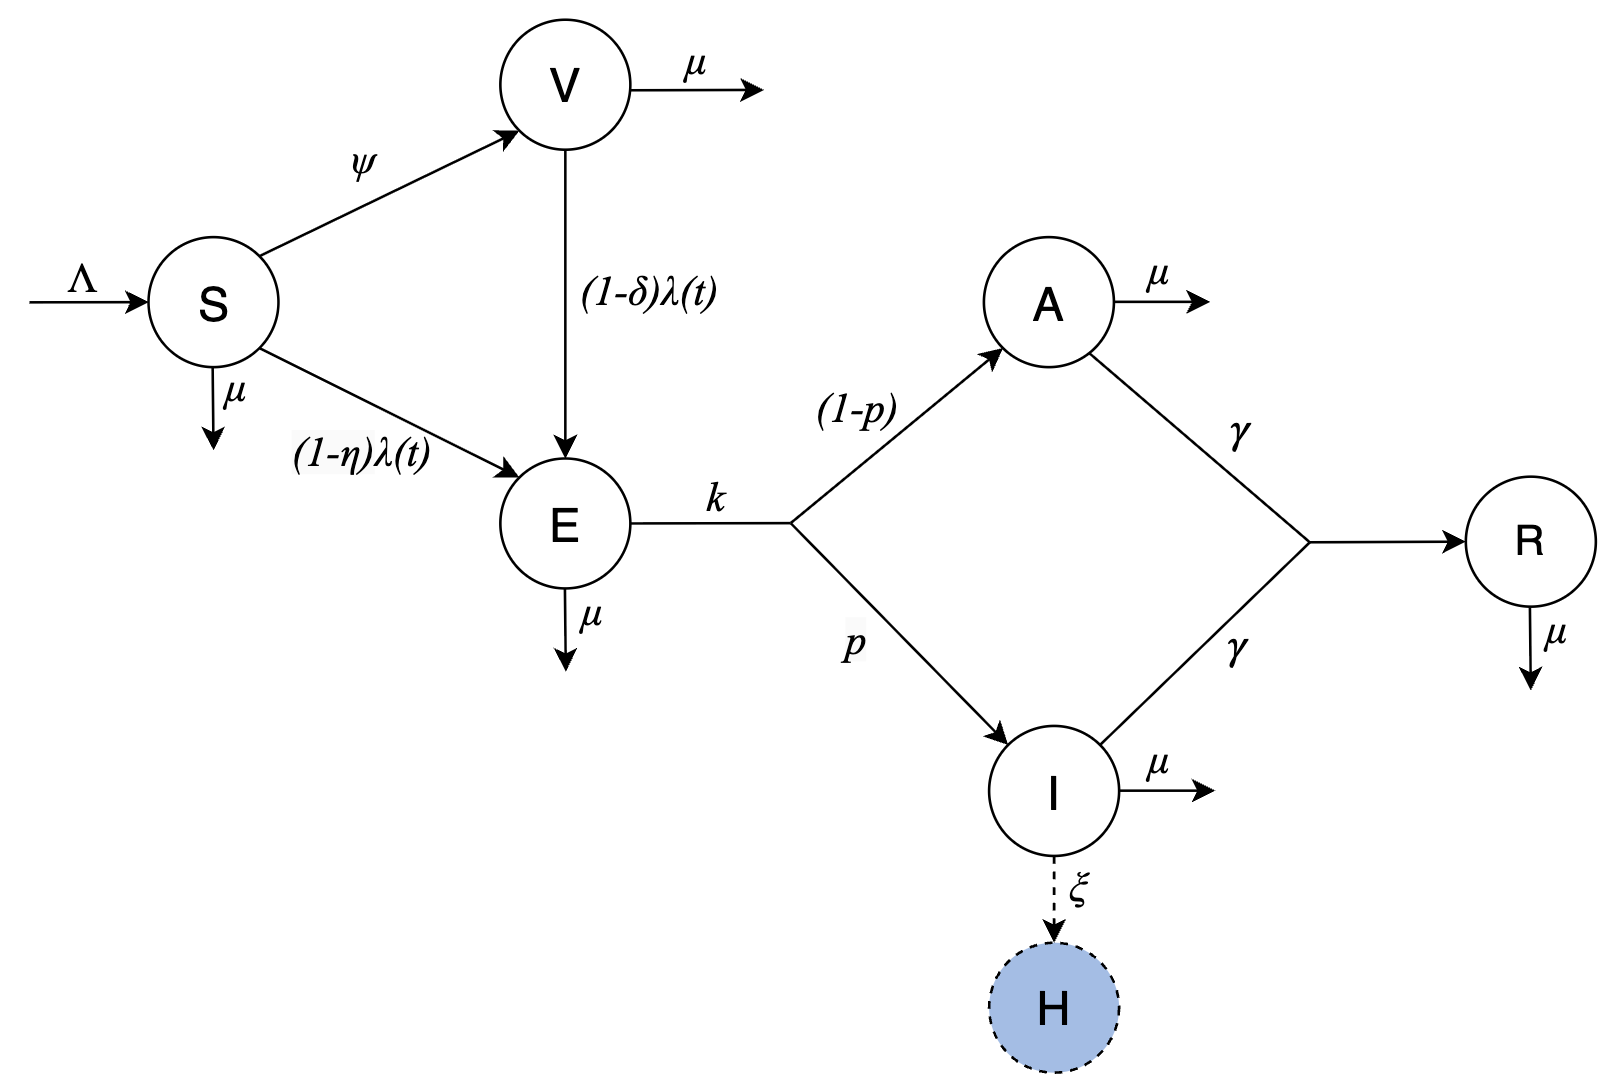
\includegraphics[width=\columnwidth]{figures/sveair-h.png} % Slightly narrower than full column
% \vspace{-2mm}
\caption{Compartmental SVEAIR epidemiological model with vaccination and masking. The `H' is not a separate compartment but denotes (observed) hospitalization numbers, typically a fraction of the true numbers from the infected compartment.}
\label{fig:sveair}
% \vspace{-4mm}
\end{figure}


\paragraph{Realistic assumptions for vaccination and masking.}
In the weekly interactive loop between individuals and the PHA (see details in Appendix~\ref{supp:weekly-loop}), masking compliance is defined based on self-reported frequency over the prior 5–7 days, classifying “all of the time” or “most of the time” as masking and other responses as non-masking, consistent with large-scale survey practice~\cite{spatiotemporal}. To account for the distinctions of vaccination and masking behaviours, the deception rates are pre-specified as 5-15\% and 40-80\%, respectively~\cite{kenya2021,Archambault2023}. 

\paragraph{Signaling game.}
%For notational convenience, we may omit the time index $t$; however, time dependency is understood to be implicit in the formulation.

For the signaling game $\mathcal{G}$, individuals communicate messages from a set $\mathcal{M}$, representing vaccination and masking status.
We encode messages as two bits $b_1b_2$, where $b_1=0$ ($1$) indicates ``Vaccinated'' (``Unvaccinated''), and $b_2=0$ ($1$) indicates ``Masking'' (``Not Masking'').
Note that $0$ denotes desirable behavior (i.e., desired by the PHA) on the part of individuals.
Reported messages may, of course, not match actual behavior, e.g., an unvaccinated or non-masking individual may claim otherwise, allowing the
capture of deception.
While we restrict attention to vaccination and masking, the framework generalizes to richer behavioral states.
Futher, we assume that only $M \leq K$ individuals in group $\mathcal{K}$ report their status. Individual types are represented by $\boldsymbol{c} = [c_1,\cdots,c_K]^T$, where $c_i=1$ denotes honesty and $c_i=0$ indicates deception. Let $g(m\mid c)$ denote the probability of sending message $m$ given type $c$. Since persistent dishonesty reduces payoffs (via penalties and social costs), deceptive individuals adopt probabilistic strategies balancing truth and misreporting. The receiver, in turn, forms beliefs about $\boldsymbol{c}$ to update the epidemiological model (Appendix~\ref{supp:epi_model}), where $\widehat{\psi}$ and $\widehat{\eta}$ denote estimated vaccination and contact rates, respectively. We now define sender and receiver payoffs.

\paragraph{Sender utility function.} Falsely claiming to be vaccinated may offer incentives, such as earning more in the workplace. Similarly, falsely stating compliance with mask-wearing may help avoid penalties imposed by the PHA. In short, while honesty about individual actions may support the societal goal of achieving zero infection rates, it could negatively impact individual payoffs. Motivated by these considerations, the expected payoffs for the sender can be defined as follows:
\begin{equation}
 % \vspace{-1mm}   
 U_s = \sum\limits_k U_s^{(k)}(c_k, m_k), \label{eq:utility}
\end{equation}
where 
\begin{equation}
\begin{aligned}
U_s^{(k)}(c_k, m_k) &= g\big(m_k = \text{``00''} \mid c_k = 0\big)(I_v + I_m) \\
& +\; g\big(m_k = \text{``01''} \mid c_k = 0\big) I_v \\
& +\; g\big(m_k = \text{``10''} \mid c_k = 0\big) I_m.
\end{aligned}
\label{eq_sender_payoff}
\end{equation}
\noindent
Here, to compute the utility, which is the incentive upon deceiving, we consider only individuals who are either not vaccinated or have not followed masking guidelines. For instance, \( g(m_k = ``00" \mid c_k=0) \) denotes a scenario where the individual has neither adopted vaccination nor masking, yet falsely communicates that they have. 
%Similarly, \( g(m_k = ``01" \mid c_k=0) \) and \( g(m_k = ``10" \mid c_k=0) \) denotes the scenarios where the individual has not adopted vaccination and masking, respectively, yet falsely communicates that they have.
In \eqref{eq_sender_payoff}, $I_v$ and $I_m$ are the incentives for communicating falsely about vaccination and masking, respectively. Maximizing solely $U_s^{(k)}(c_k,m_k)$ leads to a trivial solution where the individuals always choose to be dishonest about their strategies, since that will bring them maximum payoffs. %However, such a strategy 
This leads to  increased infection rates, closing down of businesses, and potentially punitive measures by the PHA.
Therefore, the sender in our model is interpreted as \emph{a representative population agent} rather than single strategic individuals. The population consists of a continuum of individuals facing identical incentives but potentially making heterogeneous reporting choices. Accordingly, the sender’s strategy $g(m \mid c)$ represents a population-level mixed strategy, i.e., the empirical distribution of reports generated by individuals under the same incentive structure. In this way, the sender communication strategies must represent a balance between maximizing $U_s^{(k)}(c_k,m_k)$ and minimizing these losses. 

We represent the losses as proportional to the negative of semantic accuracy, which is defined as the accuracy with which the receiver interprets the individual types from the messages communicated  and written as:
\begin{equation}
U_L(p, q) = -\frac{1}{K} \sum\limits_{i \in \mathcal{K}} \sum\limits_{j \in \mathcal{M}} p_{ij} q_{ji},
\end{equation}
where $p_{ij} = g(m_j \mid c_i)$ and $q_{ji} = q(c_i \mid m_j)$, where $q(c_i \mid m_j)$ is inference distribution at the receive side. For individuals that do not respond to the PHA, we set $p_{ij} = q_{ji} = 0$.
The sender's objective is to find a communication policy $g(m_k \mid c_k)$ by maximizing the following objective:
% \vspace{-2mm}

\begin{equation}
\mathcal{P}_1:\left[g(m_k \mid c_k)^{\ast}\right]_{\forall k} = \argmax\limits_{g(m_k \mid c_k),\, \forall k} \left( U_s - \lambda_1 U_L \right),
\end{equation}
where $\lambda_1$ is a weighting factor that represents an optimal trade-off between maximizing $U_s$ and minimizing $U_L$.


Next, to  understand  the   implications of user    misreporting, we define the control reproduction number $R_c$ as the rate at which a person can pass on the infection. The expression for $R_c$ follows  directly from \cite{ChoiJTB2020}, as
\begin{equation}
    R_c(\psi,\eta) = \underbrace{\frac{\beta k}{(k+\mu)(\gamma + \mu)}}_{R_0}\frac{(1-\delta)\psi + (1-\eta)\mu}{\psi + \mu}.
\label{eq_Rc}
\end{equation} 
A value of $R_c(\psi,\eta)>1$ represents endemic equilibrium, where the disease remains endemic in the population. Here $\beta = \beta_0(p+b(1-p))$  indicates the weighted transmission rate considering both symptomatic and asymptomatic
cases. Eqn.~\ref{eq_Rc} means that as  $R_c(\psi,\eta)$ increases, it may have severe consequences of the functioning of business, schools and other institutions. This will adversely impact the payoffs of each individual, in terms of loss of job or restrictions to the number of employees that can work, thereby reducing their salary or benefits. In practice, the reproduction number can be estimated using the available observations  \cite{ShiArxiv2025} by the PHA, such as hospitalization. To capture this estimation, we modify the sender payoffs as follows:
\begin{equation}
    \begin{aligned}
    U_s^{(k)}(c_k,m_k) &= g(m_k = ``11"\mid c_k) e^{-aR_c(\psi,\eta)}(I_v+I_m) \\ & + g(m_k = ``10"\mid c_k)e^{-aR_c(\psi,\eta)}I_{v} \\ &+ g(m_k = ``01"\mid c_k) e^{-aR_c(\psi,\eta)}I_m,
    \label{eq_sender_payoff_modified}
    \end{aligned}
\end{equation}
where $a$ is the economic factor, which is a constant coefficient that controls the slope of  the exponential  curve.

As per \eqref{eq_sender_payoff_modified}, higher $R_c(\psi,\eta)$ lowers individual payoffs. Stricter PHA measures thus reflect both rising infection rates and their economic impact on daily life. The modified sender payoffs ensure that $U_s^{(k)}$ depends not only on individual strategies but also on the PHA’s ability to predict and control the epidemic without disrupting normal activities.

%As per \eqref{eq_sender_payoff_modified}, as $R_c(\psi,\eta)$ increases, the individual payoffs reduce. Hence, when the PHA introduces stricter measures, that is indicative of the economic impact due to an exploding infection rate and hence on the day-to-day normal activities of the population. The modified sender payoffs ensure that $U_s^{(k)}$ depends not just on individual strategies but also on whether the PHA is able to accurately predict the evolution of epidemiology and hence bring it under control, without impacting the day to day activities of the population.

% \begin{figure}[t]
% \centering
% \includegraphics[width=.8\columnwidth]{AnonymousSubmission/LaTeX/sg.png}
% \caption{Illustration of signaling games.}
% \label{fig:sg}\vspace{-3mm}
% \end{figure}

\paragraph{Receiver utility function.}
The receiver's objective here is to model accurately the epidemiological ODEs in \eqref{eq_ODE} using the estimated values of $\hat{\psi}$, $\hat{\eta}$, $\hat{\lambda}$, and $\hat{\gamma}$. We define $\boldsymbol{\theta}(t) = \{\hat(\psi),\hat{\eta},\hat{\gamma},\hat{\lambda}\}$. The estimated ODE by the PHA
has the same structure as the original (ground truth one) and given in Appendix~\ref{supp:epi_model}
The estimation error will typically be given by $\abs{X(t) - \hat{X}(t)}^2$ for $X \in {S,V,E,I,A,R}$. However, the PHA cannot compute this error directly due to lack of access to ground-truth ODEs (as noted earlier). Fortunately, it can estimate hospitalizations—assumed to be a fixed fraction of infections \cite{FoxPNAS2022}—and write the estimated hospitalization count as:
%Using \eqref{eq_ODE_est}, the error between estimated and ground truth values can be defined as $\abs{X(t) - \hat{X}(t)}^2$, where $X \in \{S, V, E, I, A, R\}$. However, receiver cannot compute this error given that it does not have access to the ground-truth ODEs. Fortunately, PHA can obtain an accurate estimate of the number people who are hospitalized. It is reasonable to assume that the number of people hospitalized is equal to a fraction of the number of people infected by the virus \cite{FoxPNAS2022}. The estimated hospitalization number can be written as:
$
    H(t) = \xi I(t),
$
where $\xi$ is a constant between $0$  and $1$.
The receiver's objective is to minimize this error and thereby ensure that the protection strategies followed by it are enough to control the disease. For a given sender type and policy, the average value of the error (also called distortion) can be written as (this error should only be in terms of hospitalizations):
\begin{equation}
    D(t) = \sum\limits_{\boldsymbol{c}} p(\boldsymbol{c} \mid \boldsymbol{m}(t)) 
    \sum\limits_{\boldsymbol{\theta}(t)} p(\boldsymbol{\theta}(t) \mid \boldsymbol{c}) 
    \left| H(t) - \widehat{H}(t) \right|^2.\label{eq_error}
\end{equation}

%The above distortion can be computed by the PHA since it knows the  actual  hospitalization and the  estimated  value. 
\noindent
This distortion measure is used to add a fudge factor to the recommendation strategies which are computed based on PHA's perception of ODEs.
The PHA's recommendation of $\psi$ and $\eta$, defined as $\psi_r$ and $\eta_r$, respectively,  will be based on the estimated vaccination and social distancing rate as well as the evolution of error \eqref{eq_error}. Hence, we write:
\begin{align}
    \psi_r(t) = \widehat{\psi}(t) + \tilde{\psi}(t) \nonumber \\
    \quad \eta_r(t) = \widehat{\eta}(t) + \tilde{\eta}(t).
\end{align}
\label{eq:combined_params}
Here, the receiver aims to minimize the surprise on receiving a certain information about the epidemiological state through signaling game, while ensuring that the distortion is below a threshold. Hence, the receiver objective can be written as:
\begin{align}
    \mathcal{P}_2 : \arg\min_{p(\mathbf{c} \mid \mathbf{m})} &-\ln\left(p(\mathbf{c} \mid \mathbf{m})\right) \nonumber \\
   \textrm{s.t.}\,\,& D\leq D^{\ast},
\end{align}
\noindent  where $-\ln (p(\boldsymbol{c}\mid\boldsymbol{m}))$ is defined as the surprise, inspired from %formulations in 
other domains (e.g.,~\cite{ChristoTWCArxiv2022}).

Using the utilities defined above, we further formulate the solutions of the signaling game defined using the tuple $\left(\mathcal{K},\mathcal{C},\mathcal{M},\mathcal{M}_t,\mathcal{M}_r\right)$, where $\mathcal{C}$ is the set of user behavior types.  The Nash equilibrium (NE) strategies $\mathcal{M}_t$ (sender) and $\mathcal{M}_r$ (receiver) are such that for all $\boldsymbol{c},$ $\forall p(c_k \mid m_k) \in \mathcal{M}_r$, and $\forall g(m_k \mid c_k) \in \mathcal{M}_t$, we obtain
\begin{equation}
    \begin{aligned}
        \left[g(m_k \mid c_k)^{\ast}\right]_{\forall k} &= \argmax\limits_{g(m_k \mid c_k),\, \forall k} \left( U_s - \lambda_1 U_L \right),\\
        \left[p(\boldsymbol{c}\mid\boldsymbol{m})\right] &= \argmax\limits_{p(\boldsymbol{c}\mid\boldsymbol{m}),\boldsymbol{\theta}} \ln\left(p(\mathbf{c} \mid \mathbf{m})\right)-\lambda_2D.
    \end{aligned}
\end{equation}
%Next, we look at how to solve the transmitter and receiver strategies for the signaling game.


\paragraph{Game solution.}

%Shannon's rate-distortion theory \cite{CoverIT1991} aims to compute the solution to the following problem, which is the transmitter problem here:
%\begin{equation}
%    \mathcal{P}_1: R^{\ast}(D) = \min\limits_{-U\leq -U^{\ast}} \mathbb{I}(\boldsymbol{c};\boldsymbol{m})
%\end{equation}
A pragmatic receiver would try to compute the posterior distribution as follows:
\begin{equation}
    P_L(\boldsymbol{c}\mid \boldsymbol{m}) \propto P_S(\boldsymbol{m}\mid \boldsymbol{c}) P(\boldsymbol{c}).
\end{equation}
Here, considering parallels to Shannon's rate distortion theory \cite{CoverIT1991}, 
a pragmatic transmitter would compute a transmission strategy, so as to maximize its utility for a fixed PHA recommendations:
\begin{equation}
    P_S(\boldsymbol{m}\mid\boldsymbol{c}) \propto e^{\alpha (\sum\limits_k{U_s^k(c_k,m_k)}      -\lambda U_L(c_k,m_k))}.
\end{equation}
Further, given the transmitter (population) policy, receiver aims to minimize the surprise on receiving the messages from the population while ensuring that the distortion remains below a threshold. 
 At the receiver, we consider that $P(\boldsymbol{m})$ is known. Further, we can write the augmented Lagrangian for the receiver objective as follows:
\begin{equation}
    \begin{aligned}
&-\sum\limits_{\boldsymbol{c},\boldsymbol{m}} P(\boldsymbol{c}\mid \boldsymbol{m})P(\boldsymbol{m}) \ln P(\boldsymbol{c}\mid \boldsymbol{m}) \\
&-\lambda\sum\limits_{\boldsymbol{c},\boldsymbol{m}}P(\boldsymbol{m})p(\boldsymbol{c}\mid\boldsymbol{m})\sum\limits_{\boldsymbol{\theta}}p(\boldsymbol{\theta}\mid \boldsymbol{c})\abs{H - \widehat{H}}^2.
\end{aligned}
\label{eq_Lagrangian_receiver}
\end{equation}
The average surprise $-\sum\limits_{\boldsymbol{c},\boldsymbol{m}} P(\boldsymbol{c}\mid \boldsymbol{m})P(\boldsymbol{m}) \ln P(\boldsymbol{c}\mid \boldsymbol{m})$ is a convex function of $P(\boldsymbol{c}\mid \boldsymbol{m})$, given $\ln (x)$ is a concave function of $x$. Hence, the augmented Lagrangian in \eqref{eq_Lagrangian_receiver} is a convex function. Hence, to find out a minimizer, we take the derivative with respect to $P(\boldsymbol{c}\mid \boldsymbol{m})$. Hence, we obtain a closed form expression for the inference distribution as:
\begin{equation}
    \begin{aligned}
   & P(m) \log P(\boldsymbol{c}\mid \boldsymbol{m}) + P(m)    -\lambda \sum\limits_{\boldsymbol{\theta}}P(\boldsymbol{m})p(\boldsymbol{\theta}\mid \boldsymbol{c})\abs{H - \widehat{H}}^2
\end{aligned}
\end{equation}
\noindent
Solving for $P(\boldsymbol{c}\mid\boldsymbol{m})$ leads to the following expression.
\begin{equation}
    P(\boldsymbol{c}\mid\boldsymbol{m}) \propto e^{\frac{\lambda_2 \sum\limits_{\boldsymbol{\theta}}P(\boldsymbol{m})p(\boldsymbol{\theta}\mid \boldsymbol{c})\abs{H - \widehat{H}}^2-P(\boldsymbol{m})}{P(\boldsymbol{m})}}
\end{equation}
We compute $\boldsymbol{\theta}$, which involves the vaccination and masking strategies by the PHA using \eqref{eq:combined_params}.
From the control reproduction number $R_c(\psi,\eta)$, we can write a threshold vaccination rate as follows:
\begin{equation}
\psi_{HI} = \frac{\mu\left(R_0(1-\eta)-1\right)}{1-R_0(1-\delta)},
\end{equation}
where $1<R_0<\frac{1}{1-\delta}$. 

\section{Equilibrium Analysis}

%\subsubsection*{Scenario 1 - %$R_c(\psi,\eta) < 1$}

%\subsubsection*{Scenario %2-$R_c(\psi,\eta) > 1$} 
%\subsection*{Perfect Bayesian Nash Equilibrium}

%We define the signaling game as the tuple $\left(\mathcal{T},\mathcal{M},\mathcal{Q}\right)$, where $\mathcal{T}$ is the set of user types, $\mathcal{M}$ is the sender strategy space where $g(m\mid t)$ lies and $\mathcal{Q}$ is the strategy space of receiver where the learned distributions $\mathcal{Q}$ lies. A perfect Bayesian Nash equilibrium (NE) of the signaling game $\mathcal{G}$ is a strategy profile $()$ and posterior beliefs of the receiver about individual types $q(\boldsymbol{t})$ such that:
%\begin{equation}
%\begin{align}
%g^{\ast}(m\mid \boldsymbol{c}) & \in E_s \\
%\{\tilde{\psi},\tilde{\eta},p(\boldsymbol{\theta}(t)\mid \boldsymbol{m}(t))\} &\in \max\limits_{q}\,\,  %E_v(q_v) + E_{nv}(q_{nv})+ E_m(q_m) \\ &  E_{nm}(q_{nm}) +\alpha \mathbb{I}(\boldsymbol{\theta}(t);\boldsymbol{m}(t)) \\
%\mbox{s.t.}\,\, & \bar{e}(t)\leq %\epsilon
%\end{align}
%\end{equation}

\paragraph*{Pooling equilibrium.}

% A pooling equilibrium~\cite{HutteggerPNAS2014} is achieved when all the non-compliant are dishonest. In this case, the messages communicated do not convey any information about the strategies of the population. The PHA will have  to purely rely  on its  prior  information,  which  is  the hospitalization   number  $H(t)$.

A pooling equilibrium~\cite{HutteggerPNAS2014} is achieved when all the non-compliant individuals are dishonest. In this case, the messages communicated do not convey any information about the true behavioral strategies of the population, and the PHA must rely solely on prior information and aggregate observations, such as the hospitalization signal $H(t)$.

\begin{theorem}
\label{thm:pooling}
Suppose all non-compliant individuals strictly prefer misreporting over truthful reporting for both vaccination and masking, i.e.,
\[
U_s^{\text{lie}} > U_s^{\text{truth}}
\]
for all non-compliant types. Then there exists a pooling equilibrium in which all individuals report full compliance, i.e., $m_k = 00$ for all $k\in\mathcal{K}_c$, and the receiver’s posterior beliefs coincide with the prior distribution over types.
\end{theorem}

% In this equilibrium, reported behavioral data are uninformative, and epidemic control relies entirely on the PHA’s inference from hospitalization dynamics rather than from self-reported signals.

\paragraph{Separating equilibrium.}

% A separating equilibrium~\cite{BergstromRS2002} is achieved when all the non-compliant individuals are honest. In this cases, the messages perfectly reveal individuals’ true states, allowing PHA to infer risk accurately and select interventions such that the controlled reproduction number satisfies $R_c(\psi,\eta) < 1$, with the induced policy intensity $\widehat{\psi}$ exceeding the herd-immunity threshold $\psi_{HI}$.

A separating equilibrium \cite{BergstromRS2002} is achieved when all non-compliant individuals are honest. In this case, the reported messages perfectly reveal individuals’ true behaviors, enabling the PHA to accurately infer risk and select interventions such that the controlled reproduction number falls below one, with the induced policy intensity $\widehat{\psi}$ exceeding the herd-immunity threshold $\psi_{HI}$.

\begin{theorem}
\label{thm:separating}
If all responsive individuals report truthfully, i.e., $m_k = c_k$ for all $k\in\mathcal{K}_c$, then the signaling game admits a separating equilibrium. In this equilibrium, the PHA recovers unbiased estimates of behavioral parameters $(\psi,\eta)$ and can select policies such that
\[
R_c(\psi,\eta) < 1 \quad \text{and} \quad \widehat{\psi} > \psi_{HI},
\]
ensuring convergence to a disease-free equilibrium.
\end{theorem}

% Separating equilibria represent an idealized information regime in which signaling inefficiency does not distort epidemic control.

\paragraph{Partial pooling equilibrium.}
Departing from the extreme pooling equilibrium and the idealized separating equilibrium, a partial pooling equilibrium arises when some individuals report truthfully while others engage in deception. This is captured by the mixing factor $\alpha$. In this case, although self-reported signals are imperfect, the PHA may still extract partial information and attempt to enforce policies satisfying $R_c(\psi,\eta) < 1$ and $\widehat{\psi} > \psi_{HI}$.

\begin{theorem}
\label{thm:partial-pooling}
Consider the signaling game $\mathcal{G}$ with sender utility weight $\lambda_1$ on semantic accuracy, masking incentive $I_m$, economic factor $a$, and population type distribution $(\pi_{00}, \pi_{01}, \pi_{10}, \pi_{11})$. Define the controlled reproduction numbers $R_c(0)$ under full separation and $R_c(1)$ under full pooling, with sensitivity $\beta = \frac{dR_c}{d\alpha}\big|_{\alpha=0} > 0$.

\begin{enumerate}
    \item \textbf{Existence.} A partial pooling equilibrium with mixing probability $\alpha^* \in (0,1)$ exists if and only if the semantic weight satisfies:
    \begin{equation}
        e^{-aR_c(1)} I_m < \lambda_1 < e^{-aR_c(0)} I_m + a\beta e^{-aR_c(0)} I_m.
        \label{eq:existence-condition}
    \end{equation}
    
    \item \textbf{Characterization.} When the existence condition holds, the equilibrium mixing probability $\alpha^*$ satisfies the fixed-point equation:
    \begin{equation}
        \alpha^* = \frac{e^{-aR_c(\alpha^*)} I_m}{\lambda_1 \left(1 - p(\theta_{01} \mid m = 00)\right)},
        \label{eq:fixed-point}
    \end{equation}
    where $p(\theta_{01} \mid m = 00) = \frac{\alpha^* \pi_{01}}{\pi_{00} + \alpha^*(\pi_{01} + \pi_{10}) + \pi_{11}}$ is the posterior belief that a pooling message originated from type $\theta_{01}$.
    
    \item \textbf{Approximation.} For small deviations from separation (small $\alpha$), the equilibrium mixing probability admits the closed-form approximation:
    \begin{equation}
        \alpha^* \approx \frac{e^{-aR_c(0)} I_m}{\lambda_1 + a\beta e^{-aR_c(0)} I_m}.
        \label{eq:alpha-approx}
    \end{equation}
\end{enumerate}
\end{theorem}

\begin{proof}
See Appendix~\ref{supp:equilibrium-pooling}.
\end{proof}
The bound in  \eqref{eq:existence-condition} reveals that partial pooling emerges only when the semantic accuracy weight $\lambda_1$ lies in an intermediate range: for small $\lambda_1$ incentives dominate and all non-compliant individuals pool ($\alpha=1$); for large $\lambda_1$ accuracy dominates and all individuals separate ($\alpha=0$). %If $\lambda_1$ falls below the lower bound, incentives dominate and all non-compliant individuals pool ($\alpha = 1$). If $\lambda_1$ exceeds the upper bound, accuracy concerns dominate and all individuals separate ($\alpha = 0$). 
%The sensitivity parameter $\beta > 0$ captures how quickly the reproduction number degrades as pooling increases. Higher $\beta$ widens the existence region, making partial pooling more likely to emerge as a stable equilibrium.

% Departing from extremed pooling equilibrium and idealized separating equilibrium, partial pooling equilibrium is achieved when some individuals are honest while others may engage in deception. In this case, even with some dishonesty, PHA receives partial useful signals and tries to obtain $R_c(\psi,\eta) < 1$ and $\widehat{\psi} > \psi_{HI}$. The key question is: \emph{to what extent can deception be tolerated while still ensuring the epidemic converges to an equilibrium with negligible infections?} We decompose $\mathcal{K}$ into $\mathcal{K}_c$, the set of individuals responding to PHA queries, and $\mathcal{K}_s$, those who remain silent. The deception $\tilde{m}$ can then be characterized as:

% \begin{equation}
% \begin{aligned}
%     \tilde{m} = \frac{1}{2}\sum\limits_{k\in \mathcal{K}_c}\sum\limits_{m_k} g(m_k\mid c_k) \lVert m_k-m_k^{(\ast)} \rVert_H + \frac{1}{2}\sum\limits_{k\in \mathcal{K}_s} 2 \\ 
% = \frac{1}{2}\sum\limits_{k\in \mathcal{K}_c}\sum\limits_{m_k} g(m_k\mid c_k) \lVert m_k-m_k^{(\ast)} \rVert_H+ \abs{\mathcal{K}_s},
% \end{aligned}
% \end{equation}
% \noindent
% where $\lVert m_k-m_k^{(\ast)} \rVert_H$ is the hamming distance between communicated message and the ground truth. Using gradient descent, we optimize $\tilde{\psi}$ as follows:
% \begin{equation}
% \tilde{\psi}_t = \tilde{\psi}_{t-1} + \alpha \nabla_{\tilde{\psi}} D(t) 
% \end{equation}
% The objective is to ensure that 
% $\psi^{\ast} +\tilde{\psi} > \psi_{HI}$. Here, the population strategy that maximizes deception while ensuring $R_c(\psi,\eta) < 1$ can be written as the following problem:
% \begin{equation}
% \begin{aligned}  
% g^{\ast}(\boldsymbol{m}\mid \boldsymbol{c})=\argmax\limits_{g(\boldsymbol{m}\mid\boldsymbol{c}),\tilde{\psi}} \tilde{m}  \\
% \mbox{s.t.}\,\, \psi^{\ast} +\tilde{\psi} > \psi_{HI}
% \end{aligned}
% \end{equation}
% The resulting deception will be $\tilde{m}^{\ast} = \frac{1}{2}\sum\limits_{k\in \mathcal{K}_c}\sum\limits_{m_k} g^{\ast}(m_k\mid c_k) \lVert m_k-m_k^{(\ast)} \rVert_H + \abs{\mathcal{K}_s}$. \\

We decompose the population $\mathcal{K}$ into $\mathcal{K}_c$, the set of individuals responding to PHA queries, and $\mathcal{K}_s$, the set of silent individuals. The aggregate deception level $\tilde{m}$ is defined as:
\begin{equation}
\begin{aligned}
    \tilde{m} &= \frac{1}{2}\sum\limits_{k\in \mathcal{K}_c}\sum\limits_{m_k} g(m_k\mid c_k) \lVert m_k-m_k^{(\ast)} \rVert_H + \frac{1}{2}\sum\limits_{k\in \mathcal{K}_s} 2 \\ 
              &= \frac{1}{2}\sum\limits_{k\in \mathcal{K}_c}\sum\limits_{m_k} g(m_k\mid c_k) \lVert m_k-m_k^{(\ast)} \rVert_H + \abs{\mathcal{K}_s},
\end{aligned}
\end{equation}
where $\lVert m_k - m_k^{(\ast)} \rVert_H$ denotes the Hamming distance between the reported message and the ground-truth behavior.

Using gradient descent, the PHA updates the policy correction term $\tilde{\psi}$ as:
\begin{equation}
\tilde{\psi}_t = \tilde{\psi}_{t-1} + \alpha \nabla_{\tilde{\psi}} D(t),
\end{equation}
with the objective of ensuring $\psi^{\ast} + \tilde{\psi} > \psi_{HI}$.


% \subsubsection*{partial pooling equilibrium.}

% In this case, the deception rate is such that $R_c(\psi,\eta) > 1$. Thus, $\widehat{\psi} < \psi_{HI}$ and the population reaches an endemic equilibrium.  This means that at equilibrium, the infected people reach a constant value regardless of the PHA strategies. By substituting for $I^{\prime}=0, A^{\prime}=0$ and $R^{\prime}=0$ in \eqref{eq_ODE}, the endemic equilibrium can be calculated as 
% \begin{align}
%         E^{\ast} &= \left(V^{\ast},E^{\ast},I^{\ast},A^{\ast},R^{\ast}\right) \nonumber \\
%     &=\left(V^{\ast},\frac{\gamma+\mu}{kp}I^{\ast},I^{\ast},\frac{1-p}{p}I^{\ast},\frac{\gamma}{p\mu}I^{\ast}\right).
% \end{align}

% In the presence of an endemic equilibrium, an individual chooses deception when relative utility of deception is greater than that of being honest. This can be expressed as being deceptive when
% \begin{align}
% U_s^{(k)}(c_k,m_k) > \lambda U_L.
% \label{eq_endemic_eq_condition1}
% \end{align}
% Responding to this scenario, the PHA can choose correction factors $\tilde{\psi}$ and  $\tilde{\eta}$ such that at convergence ( i.e., at   $t=\infty$),  $D(\infty) = \sum\limits_{\boldsymbol{c}} p(\boldsymbol{c} \mid \boldsymbol{m}(\infty)) 
% \sum\limits_{\boldsymbol{\theta}(\infty)} p(\boldsymbol{\theta}(\infty) \mid \boldsymbol{c}) 
%     \left| \xi  I^{\ast} - \widehat{H}(\infty) \right|^2 $ ,   where $\widehat{H}(\infty)$ corresponds  to the   estimated hospitalization rate  under  the maximum  tolerable deception.

\section{Experimental Results}

\paragraph{Experimental settings.}
We simulate $n=50$ Monte Carlo runs of a K=10{,}000-person SVEAIR population over 26 weeks following the two stage loop of individuals reporting and PHA modeling as shown in Figure~\ref{fig:System_Model}.
Experiments span a factorial grid of equilibrium types, policy adaptivity, and experimental settings, evaluated on epidemiological, behavioral, and strategic metrics.
Details about simulation rules and evaluation procedures are provided in Appendix~\ref{supp:settings}. %We now summarize the key results of our work.

\paragraph{Interactive feedback between population and PHA drives effective epidemic control.}
To reflect the real-world settings, we consider two regimes: (1) low baseline behavioral rates ($\psi=0.005$, $\eta=0.01$), representing adverse conditions in which protective behaviors are largely neglected, and (2) high baseline behavioral rates ($\psi=0.05$, $\eta=0.10$), corresponding to more favorable conditions.
Figure~\ref{fig:rc} shows the evolution of $R_c$ across equilibria compared against a no-interaction baseline. 
Under low baseline rates (Figure~\ref{fig:rc}a), the separating and partial pooling equilibria achieve epidemic control ($R_c <1$) at week~11 and~22. Pooling fails to reach the epidemic threshold within the simulation horizon, indicating sustained transmission due to severely degraded information quality.
When initial behaviors are better (Figure~\ref{fig:rc}b), all three equilibria achieve control with different speeds: separating (week~6), partial pooling (week~8), pooling (week~13). 
In both scenarios, the no-interaction baseline remains $R_c > 1$, demonstrating that adaptive, behavior-informed feedback between the population and the PHA is essential for maintaining effective epidemic control.

\begin{figure}[htbp]
    \centering

    \begin{subfigure}[b]{0.49\columnwidth}
        \centering
        \includegraphics[width=\columnwidth]{figures/Rc_comparison_low_rate.png}
        \caption{Low baseline rates}
    \end{subfigure}
    % \hfill
    \begin{subfigure}[b]{0.49\columnwidth}
        \centering
        \includegraphics[width=\columnwidth]{figures/Rc_comparison_medium_rate.png}
        \caption{High baseline rates}
    \end{subfigure}
\vspace{-2mm}
    \caption{Controlled reproduction number ($R_c$) across equilibria vs no-interaction baseline with different initial behavioral rates.}
    \label{fig:rc} %\vspace{-4mm}
\end{figure}


% \begin{figure}[t]
%     \centering
%     \captionsetup[subfigure]{skip=0pt}

%     \begin{subfigure}[t]{0.32\columnwidth}
%         \centering
%         \includegraphics[width=\linewidth]{figures/gov_policy_sender_strategy_gmc_heatmap_separating_low_rate.png}
%         \caption{Separating}
%     \end{subfigure}
%     \hfill
%     \begin{subfigure}[t]{0.32\columnwidth}
%         \centering
%         \includegraphics[width=\linewidth]{figures/gov_policy_sender_strategy_gmc_heatmap_partial_pooling_low_rate.png}
%         \caption{Partial pooling}
%     \end{subfigure}
%     \hfill
%     \begin{subfigure}[t]{0.32\columnwidth}
%         \centering
%         \includegraphics[width=\linewidth]{figures/gov_policy_sender_strategy_gmc_heatmap_pooling_low_rate.png}
%         \caption{Pooling}
%     \end{subfigure}

%     \vspace{1mm}

%     \begin{subfigure}[t]{0.32\columnwidth}
%         \centering
%         \includegraphics[width=\linewidth]{figures/gov_policy_receiver_belief_pcm_heatmap_separating_low_rate.png}
%         \caption{Separating}
%     \end{subfigure}
%     \hfill
%     \begin{subfigure}[t]{0.32\columnwidth}
%         \centering
%         \includegraphics[width=\linewidth]{figures/gov_policy_receiver_belief_pcm_heatmap_partial_pooling_low_rate.png}
%         \caption{Partial pooling}
%     \end{subfigure}
%     \hfill
%     \begin{subfigure}[t]{0.32\columnwidth}
%         \centering
%         \includegraphics[width=\linewidth]{figures/gov_policy_receiver_belief_pcm_heatmap_pooling_low_rate.png}
%         \caption{Pooling}
%     \end{subfigure}

%     \caption{Sender strategies and receiver beliefs across equilibria.}
%     \label{fig:strategy-belief}
% \end{figure}

\begin{figure}[htbp]
    \centering
    \captionsetup[subfigure]{skip=1pt}

    % Row 1: a, d
    \begin{subfigure}[b]{0.49\columnwidth}
        \centering
        \includegraphics[width=\linewidth]{figures/gov_policy_sender_strategy_gmc_heatmap_separating_low_rate.png}
        \caption{Separating: $g(m|c)$}
    \end{subfigure}
    \hfill
    \begin{subfigure}[b]{0.49\columnwidth}
        \centering
        \includegraphics[width=\linewidth]{figures/gov_policy_receiver_belief_pcm_heatmap_separating_low_rate.png}
        \caption{Separating: $p(c|m)$}
    \end{subfigure}

    \vspace{1mm}

    % Row 2: b, e
    \begin{subfigure}[b]{0.49\columnwidth}
        \centering
        \includegraphics[width=\linewidth]{figures/gov_policy_sender_strategy_gmc_heatmap_partial_pooling_low_rate.png}
        \caption{Partial pooling: $g(m|c)$}
    \end{subfigure}
    \hfill
    \begin{subfigure}[b]{0.49\columnwidth}
        \centering
        \includegraphics[width=\linewidth]{figures/gov_policy_receiver_belief_pcm_heatmap_partial_pooling_low_rate.png}
        \caption{Partial pooling: $p(c|m)$}
    \end{subfigure}

    \vspace{1mm}

    % Row 3: c, f
    \begin{subfigure}[b]{0.49\columnwidth}
        \centering
        \includegraphics[width=\linewidth]{figures/gov_policy_sender_strategy_gmc_heatmap_pooling_low_rate.png}
        \caption{Pooling: $g(m|c)$}
    \end{subfigure}
    \hfill
    \begin{subfigure}[b]{0.49\columnwidth}
        \centering
        \includegraphics[width=\linewidth]{figures/gov_policy_receiver_belief_pcm_heatmap_pooling_low_rate.png}
        \caption{Pooling: $p(c|m)$}
    \end{subfigure}

    \caption{Sender strategies and receiver beliefs across equilibria.}
    \label{fig:strategy-belief}
\end{figure}

\paragraph{Even imperfect signals carry actionable information for the PHA about population behavior. }
Figure~\ref{fig:strategy-belief} shows sender’s strategy $g(m|c)$ and receiver’s belief $p(c|m)$ by end of period. In separating, each type reports truthfully thus receiver’s posterior perfectly recovers true types (Figure~\ref{fig:strategy-belief}a,~\ref{fig:strategy-belief}d). In pooling, all types send the same message, so the receiver’s belief collapses to the prior (Figure~\ref{fig:strategy-belief}c,~\ref{fig:strategy-belief}f). In partial pooling, while dishonest reporting by non-compliant types introduces ambiguity, informative posteriors are still recovered (Figure~\ref{fig:strategy-belief}b,~\ref{fig:strategy-belief}e). 

% \begin{figure}[htb]
%     \centering

%     % tighten space between each panel and its subcaption
%     \captionsetup[subfigure]{skip=1pt}  % requires \usepackage{subcaption}

%     \begin{subfigure}[b]{0.32\columnwidth}
%         \centering
%         \includegraphics[width=\linewidth]{figures/gov_policy_sender_strategy_gmc_heatmap_separating_low_rate.png}
%         \caption{Separating: $g(m|c)$}
%     \end{subfigure}
%     % \hfill
%     \begin{subfigure}[b]{0.32\columnwidth}
%         \centering
%         \includegraphics[width=\linewidth]{figures/gov_policy_receiver_belief_pcm_heatmap_separating_low_rate.png}
%         \caption{Separating: $p(c|m)$}
%     \end{subfigure}
    
%     \begin{subfigure}[b]{0.32\columnwidth}
%         \centering
%         \includegraphics[width=\columnwidth]{figures/gov_policy_sender_strategy_gmc_heatmap_partial_pooling_low_rate.png}
%         \caption{Partial pooling: $g(m|c)$}
%     \end{subfigure}
%     % \hfill
%     \begin{subfigure}[b]{0.32\columnwidth}
%         \centering
%         \includegraphics[width=\columnwidth]{figures/gov_policy_receiver_belief_pcm_heatmap_partial_pooling_low_rate.png}
%         \caption{Partial pooling: $p(c|m)$}
%     \end{subfigure}
    
%     % \vspace{0.3cm}
 
%     \begin{subfigure}[b]{0.32\columnwidth}
%         \centering
%         \includegraphics[width=\columnwidth]{figures/gov_policy_sender_strategy_gmc_heatmap_pooling_low_rate.png}
%         \caption{Pooling: $g(m|c)$}
%     \end{subfigure}
%     % \hfill
%     \begin{subfigure}[b]{0.32\columnwidth}
%         \centering
%         \includegraphics[width=\columnwidth]{figures/gov_policy_receiver_belief_pcm_heatmap_pooling_low_rate.png}
%         \caption{Pooling: $p(c|m)$}
%     \end{subfigure}
    
%     % \vspace{-2mm}
 
%     \caption{Sender strategies and receiver beliefs across equilibria.}
%     \label{fig:strategy-belief}     
%     %\vspace{-5mm}
 
% \end{figure}

\paragraph{Adaptive, signal-informed policy supports epidemic mitigation.}
To quantify the value of behavioral information, we benchmark our adaptive, signal-informed PHA response against a random policy that ignores the information of reports under partial pooling with low initial behavioral rates. 
Under the adaptive policy, $R_c$ falls below one at week 22, associated with lower peak hospitalization (0.0037 vs 0.0058) (Figure~\ref{fig:gov_policy}a,~\ref{fig:gov_policy}f); whereas under the random policy disease not controlled.
Adaptive feedback drives vaccination and masking intensity near their caps between weeks 3–10 (Figure~\ref{fig:gov_policy}b,~\ref{fig:gov_policy}g), producing rapid gains in coverage to roughly 60\% by week 10, compared to below 20\% under random control (Figure~\ref{fig:gov_policy}c,~\ref{fig:gov_policy}h); despite higher early deception, the overall deception rate plateaus at $0.4$ vs a stable $\sim0.5$ under random policy (Figure~\ref{fig:gov_policy}d), and more rapid growth of information content bits grow much faster, indicating more informative signals received by the PHA (Figure~\ref{fig:gov_policy}i). Sender utility rises more under adaptive control (from 0.24 to 0.34) than under random (0.31), and receiver utility is markedly higher, peaking near 6 versus staying below 1.5 (Figure~\ref{fig:gov_policy}e,~\ref{fig:gov_policy}j). Similar patterns across equilibria and initial compliance are shown in Appendix~\ref{supp: policy_comparison}, where the overall quality of control follows the expected ordering separating $>$ partial pooling $>$ pooling.
\begin{figure*}[htbp]
    \centering

    % ---------------- Row 1 ----------------
    \begin{subfigure}{0.19\textwidth}
        \centering
        \includegraphics[width=\textwidth, height=2.5cm]{figures/gov_policy_Rc_partial_pooling_low_rate.png}
        \caption{$R_c$}
    \end{subfigure}
    \hfill
    \begin{subfigure}{0.19\textwidth}
        \centering
        \includegraphics[width=\textwidth, height=2.5cm]{figures/gov_policy_vax_policy_partial_pooling_low_rate.png}
        \caption{Vaccination policy}
    \end{subfigure}
    \hfill
    \begin{subfigure}{0.19\textwidth}
        \centering
        \includegraphics[width=\textwidth, height=2.5cm]{figures/gov_policy_vax_cov_partial_pooling_low_rate.png}
        \caption{Vaccination coverage}
    \end{subfigure}
    \hfill
    \begin{subfigure}{0.19\textwidth}
        \centering
        \includegraphics[width=\textwidth, height=2.5cm]{figures/gov_policy_deception_partial_pooling_low_rate.png}
        \caption{Deception rate}
    \end{subfigure}
    \hfill
    \begin{subfigure}{0.19\textwidth}
        \centering
        \includegraphics[width=\textwidth, height=2.5cm]{figures/gov_policy_sender_utility_partial_pooling_low_rate.png}
        \caption{Sender utility}
    \end{subfigure}

    % \vspace{0.3cm}

    % ---------------- Row 2 ----------------
    \begin{subfigure}{0.19\textwidth}
        \centering
        \includegraphics[width=\textwidth, height=2.5cm]{figures/gov_policy_hospitalization_partial_pooling_low_rate.png}
        \caption{Hospitalization}
    \end{subfigure}
    \hfill
    \begin{subfigure}{0.19\textwidth}
        \centering
        \includegraphics[width=\textwidth, height=2.5cm]{figures/gov_policy_mask_policy_partial_pooling_low_rate.png}
        \caption{Mask policy}
    \end{subfigure}
    \hfill
    \begin{subfigure}{0.19\textwidth}
        \centering
        \includegraphics[width=\textwidth, height=2.5cm]{figures/gov_policy_mask_cov_partial_pooling_low_rate.png}
        \caption{Mask coverage}
    \end{subfigure}
    \hfill
    \begin{subfigure}{0.19\textwidth}
        \centering
        \includegraphics[width=\textwidth, height=2.5cm]{figures/gov_policy_info_content_bits_partial_pooling_low_rate.png}
        \caption{Information content}
    \end{subfigure}
    \hfill
    \begin{subfigure}{0.19\textwidth}
        \centering
        \includegraphics[width=\textwidth, height=2.5cm]{figures/gov_policy_receiver_utility_partial_pooling_low_rate.png}
        \caption{Receiver utility}
    \end{subfigure}
% \vspace{-2.5mm}
    \caption{Comparison of adaptive and random policies under partial pooling with low initial behavioral rates, across epidemic dynamics, policy actions, signaling behavior, and utilities.}
    \label{fig:gov_policy} %\vspace{-4mm}
\end{figure*}

% \begin{table*}[ht]
% \centering
% \renewcommand{\arraystretch}{1.2}
% \setlength{\tabcolsep}{3.5pt}
% \small
% \begin{tabular}{llrrrrc}
% \hline

% \textbf{Baseline rates} & \textbf{Outcomes} & \textbf{Separating} & \textbf{Partial pooling} & \textbf{Pooling} & \textbf{p-values} \\
% \hline
% {Low vaccination \& Low masking}
%  & Disease control       & $0.88 \pm 0.00$ & $0.50 \pm 0.00$ & $0.27 \pm 0.00$ & *** \\
%  & Deception rate        & $0.27 \pm 0.07$ & $0.52 \pm 0.02$ & $0.88 \pm 0.02$ & *** \\
%  & Sender utility        & $-0.80 \pm 1.35$ & $-2.76 \pm 1.82$ & $-3.99 \pm 0.72$ & *** \\
%  & Receiver utility      & $-4.18 \pm 1.70$ & -$3.47 \pm 0.91$ & $-3.64 \pm 0.84$ & \\
%  & Vaccination coverage  & $0.67 \pm 0.00$ & $0.73 \pm 0.00$ & $0.57 \pm 0.00$ & \\
%  & Mask coverage         & $0.90 \pm 0.00$ & $0.90 \pm 0.00$ & $0.66 \pm 0.00$ & \\
% \hline
% {Low vaccination \& High masking}
%  & Disease control       & $0.96 \pm 0.00$ & $0.85 \pm 0.00$ & $0.73 \pm 0.00$ & *** \\
%  & Deception rate        & $0.24 \pm 0.05$ & $0.40 \pm 0.02$ & $0.69 \pm 0.01$ & *** \\
%  & Sender utility        & $-0.50 \pm 0.80$ & $-0.87 \pm 1.28$ & $-2.53 \pm 0.65$ & *** \\
%  & Receiver utility      & $-4.80 \pm 1.40$ & $-1.04 \pm 1.01$ & $-0.73 \pm 0.96$ & \\
%  & Vaccination coverage  & $0.64 \pm 0.00$ & $0.90 \pm 0.00$ & $0.57 \pm 0.00$ & \\
%  & Mask coverage         & $0.90 \pm 0.00$ & $0.90 \pm 0.00$ & $0.78 \pm 0.00$ & \\
% \hline
% {High vaccination \& Low masking}
%  & Disease control       & $0.92 \pm 0.00$ & $0.73 \pm 0.00$ & $0.35 \pm 0.00$ & *** \\
%  & Deception rate        & $0.31 \pm 0.04$ & $0.44 \pm 0.02$ & $0.76 \pm 0.02$ & *** \\
%  & Sender utility        & $-0.33 \pm 1.20$ & $-1.47 \pm 1.99$ & $-3.72 \pm 0.78$ & *** \\
%  & Receiver utility      & $-7.76 \pm 1.83$ & $-0.42 \pm 0.84$ & $-1.51 \pm 0.67$ & *** \\
%  & Vaccination coverage  & $0.90 \pm 0.00$ & $0.90 \pm 0.00$ & $0.77 \pm 0.00$ & \\
%  & Mask coverage         & $0.90 \pm 0.00$ & $0.90 \pm 0.00$ & $0.69 \pm 0.00$ & \\
% \hline
% {High vaccination \& High masking}
%  & Disease control       & $0.96 \pm 0.00$ & $0.92 \pm 0.00$ & $0.85 \pm 0.00$ & *** \\
%  & Deception rate        & $0.27 \pm 0.03$ & $0.31 \pm 0.02$ & $0.57 \pm 0.01$ & *** \\
%  & Sender utility        & $-0.17 \pm 0.78$ & $-0.48 \pm 1.03$ & $-2.13 \pm 0.73$ & *** \\
%  & Receiver utility      & $-7.31 \pm 1.64$ & $-1.09 \pm 1.17$ & $-2.44 \pm 1.09$ & ** \\
%  & Vaccination coverage  & $0.90 \pm 0.00$ & $0.90 \pm 0.00$ & $0.79 \pm 0.00$ & \\
%  & Mask coverage         & $0.90 \pm 0.00$ & $0.90 \pm 0.00$ & $0.79 \pm 0.00$ & \\
% \hline
% \end{tabular}
% \caption{Comparison of epidemiological and economic outcomes across ordinal equilibrium types under different baseline behavioral settings and equilibrium types. Jonckheere–Terpstra ordered-alternative test is used to evaluate the assumption that performance declines in the order of separating $>$ partial pooling $>$ pooling. Stars indicate statistical significance ($^{*}p<0.05$, $^{**}p<0.01$, $^{***}p<0.001$).}
% \label{tab:baseline_summary}
% \end{table*}

\paragraph{Signaling game equilibria govern persistent deception patterns.}
 The overall deception rate and separate deception rates for vaccination and masking are shown in Figure~\ref{fig:deception}. Under low baseline rates (Figure~\ref{fig:deception}a), pooling exhibits the highest deception: the overall deception rate starts near 1.0 and declines toward about 0.7 by week 26. Partial pooling has intermediate deception, decreasing from 0.55 to 0.42, while separating maintains the lowest and most stable deception at 0.30 (reflection of non-responsive share). Within each equilibrium, masking deception (dotted curves) is consistently higher than vaccination deception (dashed curves), indicating that individuals are more easily misreport masking.
The same ordering persists when baseline rates are high (Figure~\ref{fig:deception}b). Partial pooling shows a pronounced decline in masking deception, falling from above 0.5 to near 0.35 by week 26. Separating remains 0.3. 
These results highlight that equilibrium structure dominates the level of dishonesty (pooling being the most deceptive), and that higher initial behavioral rates modestly reduces deceptive reporting.

\begin{figure}[t]
    \centering

    \begin{subfigure}[b]{0.4\columnwidth}
        \centering
        \includegraphics[width=\linewidth]{figures/deception_comparison_low_rate.png}
        \caption{Low baseline rates}
    \end{subfigure}
    % \hfill
    \begin{subfigure}[b]{0.4\columnwidth}
        \centering
        \includegraphics[width=\linewidth]{figures/deception_comparison_medium_rate.png}
        \caption{High baseline rates}
    \end{subfigure}

    % \vspace{-2mm}
    \caption{The deception rates across equilibria with different initial behavioral rates.}
    \label{fig:deception}
    % \vspace{-3mm}
\end{figure}


% \subsubsection{The rate at which populations adapt to PHA recommendations impact epidemic control.}

% Table \ref{tab:baseline_summary} summarizes key epidemiological and economic outcomes under scenarios of vaccination rates and masking rates. Across the ordered three equilibrium types, statistical tests confirm the trends with strong significance ($p<0.001$) for disease control, deception rate and sender utility. 
% Interestingly, vaccination and masking coverage remain high across all equilibria, indicating that the reduced utilities and elevated deception are not due to behavioral noncompliance but rather due to signaling inefficiency. 

% Looking down the rows of Table \ref{tab:baseline_summary}, we observe that higher baseline vaccination and masking rates consistently lead to improved outcomes across all equilibrium types. Disease control increases markedly from 0.27 to 0.85 under pooling—while deception rates and economic burdens (e.g., sender and receiver utility) decrease. Masking has particular strong influence on receiver utility.

% \subsubsection{High vaccination and masking incentives improve control but raise economic costs.} \td{Put this into appendix and replace with robustness experiments and stree tests.}
% \begin{figure}[htbp]
%     \centering

%      \begin{subfigure}[b]{0.49\columnwidth}
%         \centering
%         \includegraphics[width=\columnwidth]{figures/separating_disease_control_heatmap.png}
%         \caption{Disease control}
%     \end{subfigure}
%     \hfill
%         \begin{subfigure}[b]{0.49\columnwidth}
%         \centering
%         \includegraphics[width=\columnwidth]{figures/separating_receiver_distortion_heatmap.png}
%         \caption{Receiver uitility}
%     \end{subfigure}

%     \caption{Impact of incentives of vaccination and masking on disease control and receiver utility.}
%     \label{fig:incentive}
% \end{figure}
% Figure~\ref{fig:incentive} illustrates the effects of varying vaccination and masking incentives on epidemic control and the receiver utility of the PHA. When vaccination incentives are absent, individuals have little motivation to misreport, leading to truthful but low compliance that lifts the difficulty in controlling the epidemic. Figure~\ref{fig:incentive}a shows that disease control improves markedly when vaccination incentives reach 0.5, especially when masking incentives $> 1$. Across all masking incentive levels, the disease control metric suggests successful suppression of the epidemic within 26 weeks. 
% Figure~\ref{fig:incentive}b reveals the economic cost of policy incurred by the PHA. Likely when vaccination incentives are absent, small proportion of vaccinated population increases the PHA’s burden in controlling the epidemic. As vaccination incentives $\ge 0.5$, the receiver utility increases with higher incentives for both vaccination and masking, indicating a clear trade-off between public health success and associated costs.

\paragraph{Robustness of the SVEAIR–signaling-game pipeline to stress factors across equilibria.}
\begin{table}[htbp]
\centering
\caption{Stress-test outcomes for different factors across equilibria. Disease control score entries show improvements (+) or degradations (-) relative to the baseline, and peak hospitalization entries show multiplicative changes relative to the baseline peak.}
\label{tab:stress} 
\small
{%
  \setlength{\tabcolsep}{6pt} % default is ~6pt; smaller = tighter columns
  \resizebox{\linewidth}{!}{%
    \begin{tabular}{@{}lcccccc@{}} % @{} removes extra padding at left/right
    \toprule
     & \multicolumn{3}{c}{\begin{tabular}{@{}c@{}}Disease Control Score\\($\Delta$ vs Baseline)\end{tabular}}
     & \multicolumn{3}{c}{\begin{tabular}{@{}c@{}}Peak Hospitalization\\(Ratio vs Baseline)\end{tabular}} \\
    \cmidrule(lr){2-4} \cmidrule(lr){5-7}
    Factor 
      & Separating 
      & Partial pooling
      & Pooling
      & Separating 
      & Partial pooling
      & Pooling \\
    \midrule
    Infection–hospitalization ratio                  &  0.000 &  0.000 &  0.115 &  2.000 &  2.002 &  2.005 \\
    Incentives           &  0.000 & -0.077 &  0.000 &  0.998 &  1.003 &  1.002 \\
    Non-responsive share                 &  0.000 & -0.038 &  0.000 &  1.002 &  1.004 &  1.002 \\
    Vaccine Efficacy             &  0.077 &  0.423 &  0.000 &  0.551 &  0.572 &  0.616 \\
    \bottomrule
    \end{tabular}%
  }% end resizebox
}% end local tabcolsep scope
% \vspace{-2mm}
% \vspace{-3mm}
\end{table}

To validate our simulation framework, we perform a series of stress tests on key factors, including infection–hospitalization ratios (IHRs), incentives for vaccination and masking, the non-responsive share (NRS) to surveys, and vaccine efficacy. Table~\ref{tab:stress} and Figure~\ref{fig:stress} summarize how robust epidemic control is to these perturbations under all equilibria. Differences in disease control scores and ratios of peak hospitalization are reported relative to the baseline setting defined in Table~\ref{tab:param-summary}. As expected, across all equilibria, doubling IHR doubles peak hospitalization, with disease control improving only under pooling. Increases in vaccine efficacy lead to lower peak hospitalization and improved the disease control score most noticeably under partial pooling. By contrast, increasing incentives or NRS has much smaller effects because they mainly perturb how honestly people report. %The PHA’s credibility-weighted, hospitalization-driven updates can largely compensate, so vaccination and masking trajectories—and thus peak hospitalization—stay close to baseline. 


\subsection{Tolerant deception rate}

Figure \ref{fig:tolerant_deceotion} shows each combination of true vaccination and masking coverage, the largest share of individuals who can mis-report their behaviour while the epidemic remains under control ($R_c$ \textless 1). Early in the outbreak (day 60) the system is forgiving: with $\ge$60\% uptake in both levers, up to 75\% of individuals could lie and control is still maintained. As time progresses to the peak (day 90) and the post-peak phase (days 120 – 150), that “honesty buffer” contracts sharply—dropping to 55\%, 40\%, and finally 20\%—and the zero-tolerance frontier (where no deception is admissible) shifts steadily toward higher simultaneous coverage (30\%, 45\%, then 60\%). The curved contour lines indicate strong synergy: gains in one lever partly offset losses in the other, but with diminishing returns near 100\% coverage. Practically, the plots quantify when light auditing suffices (early, high-coverage regions) and when strict verification or digital proof becomes essential (late epidemic or low-coverage regimes), thereby linking data fidelity requirements directly to vaccination and masking targets over the epidemic life-cycle.

% \begin{figure}[t]
% \centering
% \includegraphics[width=\columnwidth]{AnonymousSubmission/LaTeX/tolerant-deception-2d.png} 
% \caption{Tolerant deception rate.}
% \label{fig:tolerant_deceotion}% \vspace{-4mm}
% \end{figure}


\section{Conclusion}
This paper integrates a dynamic SVEAIR epidemic model with a game-theoretic signaling framework to study how strategic misreporting of vaccination and masking affects epidemic control and policy response. %By characterizing separating, partial pooling, and pooling equilibria, we 
Our results reveal main insights. Equilibrium structure largely determines both the informational content of self-reported behaviors and the achievable quality of control: separating $>$ partial pooling $>$ pooling. %Separating equilibria preserve truthful message content, allowing the PHA to track behavior accurately and achieve $R_c<1$ fastest; pooling equilibria collapse signals to the prior, forcing policies to rely on coarse, less effective interventions.
Even with nontrivial deception, infections can still be brought under control governed by signal-informed policy. %Imperfect signals remain informative: partial pooling retains enough structure so that the PHA can infer population behavior and design policies that keep $R_c$ below one.

%(3) adaptive, behavior-informed policies substantially outperform random policies that ignore signal content. Under partial pooling with low initial behavioral rates, the adaptive controller drives $R_c$ below one, accelerates coverage gains for vaccination and masking, reduces peak hospitalization, and improves both sender and receiver utilities, while the random policy remains supercritical for much of the horizon. Stress-test experiments further show that, conditional on equilibrium structure, epidemic severity is far more sensitive to clinical severity (IHR) and vaccine performance than to moderate changes in incentives or non-response, suggesting that signaling-aware policies are robust to a broad range of behavioral perturbations.

In future work, we plan to extend our framework to state-dependent deception, and richer message spaces. %that reflect modern non-pharmaceutical intervention (NPI) channels, and more detailed economic or network-based models. 
Such extensions would allow us to study how misreporting itself spreads over contact networks, and how PHAs can design feedback rules that remain effective in the face of decentralized, adaptive behavioral responses.


% \section{Acknowledgments}

% Identification of funding sources and other support, and thanks to
% individuals and groups that assisted in the research and the
% preparation of the work should be included in an acknowledgment
% section, which is placed just before the reference section in your
% document.

% This section has a special environment:
% \begin{verbatim}
%   \begin{acks}
%   ...
%   \end{acks}
% \end{verbatim}
% so that the information contained therein can be more easily collected
% during the article metadata extraction phase, and to ensure
% consistency in the spelling of the section heading.

% Authors should not prepare this section as a numbered or unnumbered {\verb|\section|}; please use the ``{\verb|acks|}'' environment.


% %%
% %% The acknowledgments section is defined using the "acks" environment
% %% (and NOT an unnumbered section). This ensures the proper
% %% identification of the section in the article metadata, and the
% %% consistent spelling of the heading.
% % \begin{acks}
% % To Robert, for the bagels and explaining CMYK and color spaces.
% % \end{acks}


\section*{Limitations and Ethical Considerations}

Our framework makes several simplifying assumptions that can be relaxed in future work. First, the SVEAIR dynamics and the signaling layer are calibrated at the population level and do not capture individual-level heterogeneity, which may reshape epidemic trajectories, behavioral responses, and communication patterns. Second, we fix the non-responsive share and treat non-response as maximally deceptive. In practice, non-response may also arise from logistical barriers, limited access, or other non-strategic factors. Finally, we consider a single public health authority (PHA) with a fixed adaptive policy rule. Richer policy classes, including multi-agent PHAs and more diverse intervention mechanisms, may change the relative performance of equilibria and policies.

Beyond these modeling limitations, ethical considerations are important when applying strategic behavioral models to public-health decision making. Our framework does not use personally identifiable information and is intended to support population-level analysis rather than individual-level profiling or automated decision making. However, models that characterize behavioral responses could potentially be misused for manipulative communication strategies or policies that disproportionately affect certain populations. Responsible deployment requires careful validation across diverse populations, transparency in model assumptions, privacy-preserving data practices, and human oversight in policy decisions.

\section*{Generative AI Usage}

During the preparation of this manuscript, the authors used generative AI tools for limited assistance with writing refinement, grammar checking, and improving the clarity of presentation. All research ideas, mathematical formulations, experimental designs, analyses, and conclusions were developed and verified by the authors. The authors take full responsibility for the content of this paper.

% \section{Conclusion}
% This paper demonstrates how we can integrate a dynamic SVEAIR epidemic model
% with a game-theoretic signaling framework to analyze how individual misreporting of protective behaviors (vaccination and masking) affects epidemic control and policy response.
% Our results reveals that signaling game equilibria offer an effective compromise between the public health authority (PHA) and the population, enabling robust disease control even in the presence of strategic deception. Notably, active participation in vaccination or masking contributes meaningfully to suppressing disease spread, with vaccination having stronger leverage in reducing $R_c$. 

% The comparison between equilibria reveals several interesting insights.
% Separating equilibria preserve truthful message content, enabling adaptive policies to track actual behavior and achieve control more efficiently. Pooling equilibria obscure behavioral differences, forcing policies to rely on less precise interventions and thus requiring more time to bring the epidemic under control.

% In future, we plan to extend our framework to modeling state-dependent deception where incentives vary across susceptible, infected, or recovered individuals. We also plan to explore richer and overlapping message spaces to reflect modern non-pharmaceutical interventions (NPI) methodologies and reporting applications.
% Finally, coupling our signaling game with economic or network-based models would allow investigation of how misreporting spreads socially and how policy can adapt to decentralized behavioral feedback. 



\newpage
\bibliographystyle{ACM-Reference-Format}
\bibliography{signaling_games}


\newpage
\appendix
\setcounter{table}{0}
\renewcommand{\thetable}{A\arabic{table}}

\setcounter{figure}{0}
\renewcommand{\thefigure}{A\arabic{figure}}

\section{Epidemiological Model}
\label{supp:epi_model}
The epidemiological model studied in this paper is given by:

\begin{align}
S^{\prime}(t) &= \Lambda - \lambda(t)(1-\eta)S(t) - (\psi + \mu)S(t), \nonumber \\
V^{\prime}(t) &= \psi S(t) - \lambda(t)(1-\delta)V(t) - \mu V(t), \nonumber \\
E^{\prime}(t) &= \lambda(t)\left((1-\eta)S(t) + (1-\delta)V(t)\right)- (k+\mu)E(t), \nonumber \\
A^{\prime}(t) &= k(1-p)E(t) - (\gamma+\mu)A(t), \nonumber \\
I^{\prime}(t) &= kpE(t) - (\gamma+\mu)I(t), \nonumber \\
R^{\prime}(t) &= \gamma (A(t) + I(t)) - \mu R(t), \label{eq_ODE}
\end{align}
where $X^{\prime}(t) = \frac{d X(t)}{d t}$. We define the vaccination rate as $\psi\ (0\leq \psi \leq 1)$ and the masking rate as $\eta\ (0\leq \eta \leq 1)$, indicating that susceptible individuals reduce the contact rate by a fraction of $\eta$. 
Vaccine efficiency is described using the factor $\delta$, which quantifies the rate of reduction in infection rate for vaccinated individuals. 
Disease-free individuals enter the susceptible class through birth or immigration at a constant rate $\Lambda$ and their natural death rate is denoted by $\mu$. It is assumed that susceptible individuals become infected at a rate of $\lambda(t) = \frac{\beta_0(t)(I(t)+bA(t))}{K(t)}$. Here, $\beta_0$ is the transmission rate, $b$ is the rate of relative infectiousness of asymptomatic cases compared to symptomatic cases, and $K(t) = S(t) + V(t) + E(t) + I(t) + A(t)+R(t)$. We define $1/k$ as the duration of the latent period, which is defined as the time between when a person is exposed to the disease and when they become infectious. We also assume that a proportion $p$ of infected individuals become symptomatic.  Both symptomatic and asymptomatic individuals are assumed to recover at a rate of $\gamma$. 

Likewise, the ODE model estimated by the receiver (i.e., the PHA) is given by:

\begin{align}
\hat{S}'(t) &= \Lambda - \hat{\lambda}(t) (1 - \hat{\eta}) \hat{S}(t) - (\hat{\psi} + \mu) \hat{S}(t), \nonumber \\
\hat{V}'(t) &= \hat{\psi} \hat{S}(t) - \hat{\lambda}(t) (1 - \delta) \hat{V}(t) - \mu \hat{V}(t), \nonumber \\
\hat{E}'(t) &= \hat{\lambda}(t) \left((1 - \hat{\eta}) \hat{S}(t) + (1 - \delta) \hat{V}(t)\right) - (k + \mu) \hat{E}(t), \nonumber \\
\hat{A}'(t) &= k(1 - p) \hat{E}(t) - (\hat{\gamma} + \mu) \hat{A}(t), \nonumber \\
\hat{I}'(t) &= kp \hat{E}(t) - (\hat{\gamma} + \mu) \hat{I}(t), \nonumber \\
\hat{R}'(t) &= \hat{\gamma} (\hat{A}(t) + \hat{I}(t)) - \mu \hat{R}(t).
\label{eq_ODE_est}
\end{align}

%The ODE model as described by Eq.~\ref{eq_ODE} is illustrated by the logical flow diagram of Fig.~\ref{fig:sveair}. Next, we discuss in detail the specifics of signaling game. For notational convenience, we may omit the time index $t$; however, time dependency is understood to be implicit in the formulation.


\section{Behavioral Types}
Table~\ref{tab:truth-table-9types}
denote 9 behavioral types of individuals capturing their true status and how they report their vaccination and/or masking status. To interpret the `True Status' column, note that 0 indicates compliance and 1 indicates non-compliance. The first number in the True Status column is meant for vaccination status and the second number denotes masking status. 
In row 2, for instance, the true status is 01, i.e., the individual is vaccinated but not masking.
However, this individual reports 00 (i.e., they are honest about their vaccination status but deceptive about their masking status). The number of possible types is not a true cross-product because individuals who are masked or who are vaccinated are assumed to have no incentive to lie about their status. Thus there is a `Deceptive' value in a row only if the corresponding entry in True Status is a 1 (i.e., non-compliance).

\begin{table}[t]
\centering
\caption{Nine behavioral types defined in terms of how people with different compliance combinations report truthfully or deceive about their vaccination and/or masking status. (See A.2 for explanation.)}
\label{tab:truth-table-9types}
\begin{tabular}{l|l|l|l}
\hline
\textbf{Type} & \textbf{True status} & \textbf{Vaccine report} & \textbf{Mask report} \\
\hline
$T_1$ & 00 & 0 (Honest) & 0 (Honest) \\
$T_2$ & 01 & 0 (Honest) & 0 (Deceptive) \\
$T_3$ & 01 & 0 (Honest) & 1 (Honest) \\
$T_4$ & 10 & 0 (Deceptive) & 0 (Honest) \\
$T_5$ & 10 & 1 (Honest) & 0 (Honest) \\
$T_6$ & 11 & 0 (Deceptive) & 0 (Deceptive) \\
$T_7$ & 11 & 0 (Deceptive) & 1 (Honest) \\
$T_8$ & 11 & 1 (Honest) & 0 (Deceptive) \\
$T_9$ & 11 & 1 (Honest) & 1 (Honest) \\
\hline
\end{tabular}
\end{table}


% \section{Controlled $\mathcal{R}_c$ Derivation via the Next-Generation Matrix}
% \label{rc_derivation}
% We derive the controlled reproduction number $\mathcal{R}_c$ for the $\text{SVEAIR}$ model under vaccination, masking, and distancing. 
% Let the compartmental states be $(\hat{S}, \hat{V}, \hat{E}, \hat{A}, \hat{I}, \hat{R})$, with total population 
% $N = \hat{S} + \hat{V} + \hat{E} + \hat{A} + \hat{I} + \hat{R}$. 
% The controlled dynamics are given by Eq.~(23).

% \paragraph{Step 1. Disease-Free Equilibrium (DFE).}
% At the DFE, $\hat{E}^*=\hat{A}^*=\hat{I}^*=0$ and $\hat{S}^*=(1-\hat{\psi})N$. 
% Linearizing the infected subsystem $(\hat{E},\hat{A},\hat{I})$ around the DFE gives
% \begin{equation}
% \frac{d}{dt}
% \begin{bmatrix}
% \hat{E}\\[2pt]\hat{A}\\[2pt]\hat{I}
% \end{bmatrix}
% = \mathcal{F} - \mathcal{V}.
% \end{equation}

% \paragraph{Step 2. New-infection and transition terms.}
% At the DFE,
% \begin{align}
% \begin{aligned}
% \mathcal{F} &=
% \begin{bmatrix}
% \hat{\beta}(1-\hat{\eta})(1-\delta)(1-\hat{\psi})(\hat{I} + \kappa \hat{A})\\[4pt]
% 0\\[4pt]
% 0
% \end{bmatrix},\\[10pt]
% \mathcal{V} &=
% \begin{bmatrix}
% (k+\mu)\hat{E}\\[4pt]
% -(1-p)k\hat{E} + (\hat{\gamma}+\mu)\hat{A}\\[4pt]
% - pk\hat{E} + (\hat{\gamma}+\mu)\hat{I}
% \end{bmatrix}.
% \end{aligned}
% \end{align}

% \paragraph{Step 3. Jacobians at the DFE.}
% \begin{align}
% \begin{aligned}
% F &=
% \begin{bmatrix}
% 0 & \hat{\beta}(1-\hat{\eta})(1-\delta)(1-\hat{\psi})\kappa & \hat{\beta}(1-\hat{\eta})(1-\delta)(1-\hat{\psi})\\[4pt]
% 0 & 0 & 0\\[4pt]
% 0 & 0 & 0
% \end{bmatrix},\\[10pt]
% V &=
% \begin{bmatrix}
% k+\mu & 0 & 0\\[4pt]
% -(1-p)k & \hat{\gamma}+\mu & 0\\[4pt]
% - pk & 0 & \hat{\gamma}+\mu
% \end{bmatrix}.
% \end{aligned}
% \end{align}

% \paragraph{Step 4. Next-Generation Matrix and Controlled $\mathcal{R}_c$.}
% The next-generation matrix is
% \begin{equation}
% K = F V^{-1}, \qquad
% \mathcal{R}_c = \rho(K),
% \end{equation}
% where $\rho(\cdot)$ denotes the spectral radius. 
% After simplification,
% \begin{align}
% \mathcal{R}_c 
% &= (1-\hat{\psi})(1-\hat{\eta})(1-\delta)\,\hat{\beta}
%    \!\left(
%    \frac{p}{\hat{\gamma}+\mu}
%    + \kappa\,\frac{1-p}{\hat{\gamma}+\mu}
%    \right).
% \end{align}

% \paragraph{Interpretation.}
% Equation~(X.1) shows that $\mathcal{R}_c$ decreases multiplicatively with control measures:
% \begin{itemize}
%   \item $(1-\hat{\psi})$ reduces susceptibility via vaccination,
%   \item $(1-\hat{\eta})$ attenuates transmission via masking,
%   \item $(1-\delta)$ reduces contact rates via distancing.
% \end{itemize}
% The disease-free equilibrium is stable when $\mathcal{R}_c < 1$.

% \section{Effective Transmission Term under Masking and Vaccination}

% From Eq.~(22), the dynamics of the susceptible and vaccinated compartments are:
% \begin{align}
% S'(t) &= \Lambda - \lambda(t)(1-\eta)S(t) - (\psi + \mu)S(t), \\
% V'(t) &= \psi S(t) - \lambda(t)(1-\delta)V(t) - \mu V(t),
% \end{align}
% where $\lambda(t) = \beta_0(t)\dfrac{I(t) + bA(t)}{K(t)}$ is the force of infection. 
% Here, $\beta_0$ is the baseline transmission rate, $\eta$ is the masking rate 
% ($0 \le \eta \le 1$) describing the fraction of transmission reduction due to masking, 
% $\psi$ is the vaccination rate, and $\delta$ is vaccine efficacy (the reduction in susceptibility 
% for vaccinated individuals).

% % \vspace{0.5em}
% \noindent\textbf{Step 1. Effective susceptibility.} 
% At any time $t$, the unvaccinated fraction $(1-\psi)$ remains fully susceptible, 
% while the vaccinated fraction $\psi$ has its susceptibility reduced by $(1-\delta)$. 
% The average (population-level) residual susceptibility is therefore
% \begin{equation}
% S_{\text{eff}} = (1-\psi) + (1-\delta)\psi = 1 - \psi\delta.
% \label{eq:Seff}
% \end{equation}

% % \vspace{0.5em}
% \noindent\textbf{Step 2. Incorporating masking.}
% Masking reduces transmission probability or contact rate by a multiplicative factor $(1-\eta)$. 
% Hence, the overall effective transmission coefficient becomes:
% \begin{equation}
% \beta_{\text{eff}} = \beta_0 (1-\eta)[1-\psi\delta].
% \label{eq:beta_eff}
% \end{equation}

% % \vspace{0.5em}
% \noindent\textbf{Step 3. Interpretation.}
% \begin{itemize}
%     \item $\beta_0$ --- baseline transmission rate in the absence of interventions.
%     \item $(1-\eta)$ --- residual transmission after masking or contact-rate reduction.
%     \item $[1-\psi\delta]$ --- residual susceptibility after vaccination, i.e., 
%     the proportion of individuals who remain susceptible despite vaccination.
% \end{itemize}
% The product in Eq.~\eqref{eq:beta_eff} therefore represents the \emph{effective transmission strength} 
% under masking and vaccination.

% % \vspace{0.5em}
% \noindent\textbf{Step 4. Effective force of infection.}
% The effective population-level force of infection can thus be expressed as:
% \begin{equation}
% \lambda_{\text{eff}}(t) = 
% \beta_0 (1-\eta)[1-\psi\delta]\,
% \dfrac{I(t) + bA(t)}{K(t)}.
% \label{eq:lambda_eff}
% \end{equation}

% % \vspace{0.5em}
% \noindent\textbf{Step 5. Identifiability implication.}
% Because masking $(1-\eta)$ and vaccination $[1-\psi\delta]$ appear multiplicatively 
% in Eq.~\eqref{eq:lambda_eff}, their effects on epidemic outcomes 
% (e.g., cases or hospitalizations) are statistically confounded. 
% An increase in masking can be offset by a decrease in vaccination and vice versa, 
% leading to the same epidemic trajectory. 
% Hence, only the combined quantity
% \begin{equation}
% \chi = (1-\eta)[1-\psi\delta]
% \label{eq:chi}
% \end{equation}
% is structurally identifiable from observable data.

\section{Equilibrium Characterization}
\label{supp:equilibrium}
\subsection{Pooling equilibrium}
In pooling, all types send the same message $m^* = 00$ (claim full compliance).
Here, the sender Strategy can be written as:
\begin{equation}
    g^*(m|c) = 
\begin{cases}
1 & \text{if } m = 00 \\
0 & \text{otherwise}
\end{cases}
\quad \forall c
\end{equation}
Receiver Belief  can be written as:
\begin{equation}
    p^*(c \mid m = 00) = p(c) \quad \text{(prior probability)}
\end{equation}
The PHA learns nothing from messages and must rely on rior population compliance rates and observable hospitalizations $H(t)$.
Pooling exists when deviating to truth-telling is not profitable. For a non-compliant individual ($c \neq 00$):
$
U_s(m = 00 \mid c) \geq U_s(m = c \mid c)$.
This holds when incentives dominate semantic accuracy. 
$
I_v + I_m \succ \frac{1}{|M|} \cdot \frac{1}{K}$. 

\[
e^{-a R_c^{\text{pooling}}} (I_v + I_m) > \lambda_1 \cdot K^{-1}
\]
\emph{Receiver's Best Response:}
Under pooling, the PHA must estimate $\hat{\omega}, \hat{\epsilon}$ from hospitalizations alone, i.e.,
\[
\hat{\psi}(t) = \omega_0 + \psi_{\Delta}(t)
\]
\[
\hat{\eta}(t) = \eta + \eta_{\Delta}(t),
\]
Where corrections $\psi{\Delta}, \eta{\Delta}$ solve:
\[
\min_{\psi_{\Delta}, \eta_{\Delta}} \left| H(t) - \xi\hat{I}(t; \psi + \psi_{\Delta}, \eta + \eta_{\Delta}) \right|^2
\]
subject to distortion constraint:
$
D(t) \leq D^*$.
\emph{Deception Rate}
can be written as:
$\tilde{m}^* = \frac{1}{2} \sum_{k \in K_c} \| m_k - c_k \|_H + |K_s|
$, where $\| m_k - c_k \|_H$ is Hamming distance. In pure pooling with $m = 00$ for all, we obtain
$
\tilde{m}^* = \frac{1}{2} |K_c| \cdot \mathbb{E}[\| 00 - c \|_H] + |K_s|
$.
If population has baseline rates $(\psi^\ast, \eta^\ast)$ (round truth), then we get
\begin{equation}
\begin{aligned}
\tilde{m}^* &= |K_c|(1 - \psi^\ast)(1 - \eta^\ast) + \frac{1}{2}|K_c|\psi^\ast(1 - \eta^\ast) \\ &+\frac{1}{2}|K_c|(1-\psi^\ast) \eta^\ast+  |K_s|.
\end{aligned}
\end{equation}

\subsection{Partial pooling equilibrium}
\label{supp:equilibrium-pooling}
Here, some users separate and others pool, with mixing probability defined as $\alpha$. We consider a simplistic model of sender strategy as written below:
\begin{equation}
    g^*(m|c) =
\begin{cases}
1 & \text{if } c = 00 \text{ and } m = 00 \\
\alpha & \text{if } c \in \{01,10\} \text{ and } m = 00 \\
1-\alpha & \text{if } c \in \{01,10\} \text{ and } m = c \\
1 & \text{if } c = 11 \text{ and } m = 00 \\
0 & \text{otherwise}
\end{cases}
\end{equation}
Let:
$\pi_{00}$ represents fraction truly compliant (vaccinated + masking),
 $\pi_{01}$ represents fraction vaccinated but not masking
$\pi_{10}$  represents fraction masking but not vaccinated, and 
 $\pi_{11}$  represents  fraction non-compliant on both, with
$
\pi_{00} + \pi_{01} + \pi_{10} + \pi_{11} = 1.
$ Given mixing probability $\alpha$, the proportion sending each message becomes,
\begin{equation}
\begin{aligned}
P(m = 00) &= \pi_{00} + \alpha(\pi_{01} + \pi_{10}) + \pi_{11}\\
P(m = 01) &= (1 - \alpha)\pi_{01}\\
P(m = 10) &= (1 - \alpha)\pi_{10}\\
P(m = 11) &= 0 \quad \text{(no one admits full non-compliance)}    
\end{aligned}
\end{equation}
Using Bayes' rule, when PHA receives $m = 00$, and $\theta_{ij}$ representing the estimate of type $``ij"$,
\begin{equation}\begin{aligned}
p(\theta_{00} \mid m = 00) &= \frac{\pi_{00}}{\pi_{00} + \alpha(\pi_{01} + \pi_{10}) + \pi_{11}}\\
p(\theta_{01} \mid m = 00) &= \frac{\alpha \pi_{01}}{\pi_{00} + \alpha(\pi_{01} + \pi_{10}) + \pi_{11}}\\
p(\theta_{10} \mid m = 00) &= \frac{\alpha \pi_{10}}{\pi_{00} + \alpha(\pi_{01} + \pi_{10}) + \pi_{11}}\\
p(\theta_{11} \mid m = 00) &= \frac{\pi_{11}}{\pi_{00} + \alpha(\pi_{01} + \pi_{10}) + \pi_{11}}\end{aligned}
\end{equation}
The PHA estimates vaccination rate as:
\begin{equation}
\begin{aligned}
\hat{\psi}(\alpha) &= \pi_{00} + \pi_{01} + \alpha\pi_{10}+ \pi_{11}
\end{aligned}
\end{equation}
\begin{equation}
\hat{\eta}(\alpha) = \pi_{00} + \pi_{10} + \alpha\pi_{01}+ \pi_{11}
\end{equation}
Similarly for masking:
\begin{equation}
\hat{\epsilon}(\alpha) = P(m = 00) \cdot \frac{\pi_{00} + \alpha \pi_{10}}{\pi_{00} + \alpha(\pi_{01} + \pi_{10}) + \pi_{11}} + (1 - \alpha)\pi_{10}
\end{equation}
\textit{Key observation:} $\hat{\psi}(\alpha)$ and $\hat{\eta}(\alpha)$ are overestimates of true compliance because of pooling. From eq.~\eqref{eq_Rc}, $R_c(\alpha) = R_c(\hat{\psi},\hat{\eta})$. As $\alpha$ increases (indicating more pooling), $\hat{\psi}(\alpha)$ and $\hat{\eta}(\alpha)$ both increase because the PHA believes more individuals are vaccinated and masking, even though true compliance remains unchanged; consequently, the PHA under-responds, leading to an increase in $R_c(\alpha)$. The semantic accuracy term can be written when the actual type is $\theta_{01}$ as:
\begin{equation}
U_{L,\text{pool}}^{01}(\alpha) = \alpha \cdot p(\theta_{01} \mid m = 00) + (1 - \alpha)
\end{equation}
For type $\theta_{01}$ pooling:
\begin{equation}
U^{01}_{\text{pool}}(\alpha) = e^{-a R_c(\alpha)} I_m + \lambda_1 \cdot \big[ \alpha \cdot p(\theta_{01} \mid m = 00) + (1 - \alpha) \big],
\end{equation}
and for type $\theta_{01}$ separating:
\begin{equation}
U^{01}_{L,\text{sep}} = 0 + \lambda_1 \cdot 1 = \lambda_1
\end{equation}
For optimal mixing,
we need
$U^{01}_{\text{pool}}(\alpha^*) = U^{01}_{\text{sep}}. $ This leads to:
\begin{equation}
e^{-a R_c(\alpha^*)} I_m + \lambda_1 \big[ \alpha^* \cdot p(\theta_{01} \mid m = 00) + (1 - \alpha^*) \big] = \lambda_1
\end{equation}
Simplifying this, we obtain
\begin{equation}
\alpha^* = \frac{e^{-a R_c(\alpha^*)} I_m}{\lambda_1 \big[ 1 - p(\theta_{01} \mid m = 00) \big]}.
\end{equation}
Substituting Bayes' rule, we obtain:
\begin{equation}
e^{-a R_c(\alpha^*)} I_m = \lambda_1 \alpha^* \left[ 1 - \frac{\alpha^* \pi_{01}}{\pi_{00} + \alpha^*(\pi_{01} + \pi_{10}) + \pi_{11}} \right]
\end{equation}
This is an implicit equation in $\alpha^*$ because $R_c(\alpha^*)$ depends on $\alpha^*$ and the right-hand side contains $\alpha^*$ in a nonlinear way. Therefore, it generally requires a numerical solution. For small deviations from separation, we use a linear approximation:
\begin{equation}
R_c(\alpha) \approx R_c(0) + \beta \alpha
\end{equation}
where
\begin{equation}
\beta = \left. \frac{d R_c}{d \alpha} \right|_{\alpha = 0} > 0
\end{equation}
Similarly, the conditional probability can be approximated as:
\begin{equation}
p(\theta_{01} \mid m = 00) \approx \frac{\alpha \pi_{01}}{\pi_{00} + \pi_{11}}
\end{equation}
Then, using the linear approximation for $R_c(\alpha)$ and ignoring higher-order terms, we have:
\begin{equation}
e^{-a [R_c(0) + \beta \alpha]} I_m \approx \lambda_1 \alpha \left[ 1 - \frac{\alpha \pi_{01}}{\pi_{00} + \pi_{11}} \right]
\end{equation}
For small $\alpha$, ignoring $\alpha^2$ terms, this simplifies to:
\begin{equation}
e^{-a R_c(0)} (1 - a \beta \alpha) I_m \approx \lambda_1 \alpha
\end{equation}
Rearranging terms gives:
\begin{equation}
e^{-a R_c(0)} I_m \approx \lambda_1 \alpha + a \beta e^{-a R_c(0)} I_m \cdot \alpha
\end{equation}
Finally, solving for $\alpha^*$ yields:
\begin{equation}
\alpha^* \approx \frac{e^{-a R_c(0)} I_m}{\lambda_1 + a \beta e^{-a R_c(0)} I_m}
\end{equation}

\subsubsection{Existence conditions}
For partial pooling equilibrium to exist, we require $0 < \alpha^* < 1$. To find a lower bound, consider when pure separation ($\alpha = 0$) is not an equilibrium. At $\alpha = 0$, suppose type $\theta_{01}$ deviates to pool. The utility from deviating is:
\begin{equation}
\begin{aligned}
U_{L,\text{pool}}^{01}(\alpha=0)
&= e^{-a R_c(0)} I_m + \lambda_1 \big[(1 - 0) + 0 \cdot 0 \big] \\
&= e^{-a R_c(0)} I_m + \lambda_1 .
\end{aligned}
\end{equation}
The utility from separating is:
\begin{equation}
U_{L,\text{sep}}(\alpha=0) = \lambda_1
\end{equation}
For separation to be unstable, we need:
\begin{equation}
e^{-a R_c(0)} I_m + \lambda_1 > \lambda_1
\end{equation}
This simplifies to:
\begin{equation}
e^{-a R_c(0)} I_m > 0
\end{equation}
which is always true, implying that pure separation cannot be an equilibrium when $I_m > 0$. To determine when pure pooling ($\alpha = 1$) is not an equilibrium, note that at $\alpha = 1$, everyone pools. The conditional probability is:
\begin{equation}
p(\theta_{01} \mid m = 00) = \frac{\pi_{01}}{\pi_{00} + \pi_{01} + \pi_{10} + \pi_{11}} = \pi_{01}
\end{equation}
The utility from pooling is:
\begin{equation}
\begin{aligned}
U_{L,\text{pool}}(1) &= e^{-a R_c(1)} I_m + \lambda_1 \big[(1 - 1) + 1 \cdot \pi_{01}\big]\\& = e^{-a R_c(1)} I_m + \lambda_1 \pi_{01}
\end{aligned}
\end{equation}
The utility from deviating to separate is:
\begin{equation}
U_{L,\text{sep}} = \lambda_1
\end{equation}
For pooling to be unstable (deviation profitable), we require:
\begin{equation}
e^{-a R_c(1)} I_m + \lambda_1 \pi_{01} < \lambda_1
\end{equation}
Since $(1 - \pi_{01}) \leq 1$, the condition for pooling to be unstable simplifies to:
\begin{equation}
e^{-a R_c(1)} I_m < \lambda_1
\end{equation}
From the approximation
\begin{equation}
\alpha^* \approx \frac{e^{-a R_c(0)} I_m}{\lambda_1 + a \beta e^{-a R_c(0)} I_m},
\end{equation}
for $\alpha^* < 1$, we require:
\begin{equation}
e^{-a R_c(0)} I_m < \lambda_1 + a \beta e^{-a R_c(0)} I_m.
\end{equation}
Rearranging gives:
\begin{equation}
e^{-a R_c(0)} I_m (1 - a \beta) < \lambda_1.
\end{equation}

For small $a \beta$, this implies:
\begin{equation}
\lambda_1 > e^{-a R_c(0)} I_m - a \beta e^{-a R_c(0)} I_m.
\end{equation}

Combining this lower bound on $\lambda_1$ with the upper bound from pooling instability, we obtain:
\begin{equation}
e^{-a R_c(1)} I_m < \lambda_1 < e^{-a R_c(0)} I_m + a \beta e^{-a R_c(0)} I_m.
\label{bounds_partialpooling}
\end{equation}
From \eqref{bounds_partialpooling} we infer the following conclusions.
The semantic weight $\lambda_1$ must lie in a Goldilocks zone for mixed to exist. If $\lambda_1$ is too low (below the lower bound), semantic accuracy does not matter much, incentives dominate, and everyone pools ($\alpha = 1$), resulting in a full pooling equilibrium. If $\lambda_1$ is too high (above the upper bound), semantic accuracy matters a lot, people value being understood correctly, and everyone separates ($\alpha = 0$), leading to a separating equilibrium.
If $\lambda_1$ is just right (within the window), there is a trade-off between incentives and accuracy, and mixed occurs with $0 < \alpha^* < 1$. In this case, some individuals lie while others tell the truth, creating a stable mixing equilibrium.

\subsection{Tolerance frontiers}

In partial pooling equilibrium, the key question is: \emph{to what extent can deception be tolerated while still ensuring the epidemic converges to an equilibrium with negligible infections?}

\begin{theorem}[Partial Pooling and Tolerable Deception]
\label{thm:partial}
There exists a partial pooling equilibrium in which some non-compliant individuals misreport while others report truthfully if and only if the induced deception level $\tilde{m}$ remains below a critical tolerance threshold $\tilde{m}_{\max}$ such that the PHA can select policies satisfying
\[
R_c(\psi,\eta) < 1 \quad \text{and} \quad \widehat{\psi} > \psi_{HI}.
\]
In this regime, epidemic control is preserved despite strategic misreporting.
\end{theorem}

The population strategy that maximizes deception while preserving epidemic control can be expressed as:
\begin{equation}
\begin{aligned}
g^{\ast}(\boldsymbol{m}\mid \boldsymbol{c})
= \argmax_{g(\boldsymbol{m}\mid\boldsymbol{c}),\,\tilde{\psi}} \ \tilde{m}
\quad
\text{s.t.}\quad
\psi^{\ast} + \tilde{\psi} > \psi_{HI}.
\end{aligned}
\end{equation}

The resulting equilibrium deception level is given by:
\begin{equation}
\begin{aligned}
\tilde{m}^{\ast}
=
\frac{1}{2}\sum_{k\in \mathcal{K}_c}\sum_{m_k} g^{\ast}(m_k\mid c_k)\lVert m_k-m_k^{(\ast)} \rVert_H
+ |\mathcal{K}_s|.
\end{aligned}
\end{equation}

This characterization defines a \emph{tolerance frontier} that quantifies how much strategic misreporting can be absorbed before epidemic control breaks down.

We further decompose the deception into vaccination and masking components.
Let $h_v(m_k,m_k^{(*)}) \in \{0,1\}$ and $h_\eta(m_k,m_k^{(*)}) \in \{0,1\}$
denote the Hamming distance restricted to the vaccination bit and the
masking bit, respectively. Then the vaccination deception $\tilde{m}^{(v)}$
and masking deception $\tilde{m}^{(\eta)}$ can be written as
\begin{align}
\tilde{m}^{(v)}
  &= \sum_{k \in \mathcal{K}_c} \sum_{m_k} g(m_k \mid c_k)\,
     h_v\!\bigl(m_k, m_k^{(*)}\bigr)
     + \abs{\mathcal{K}_s}, \label{eq:vax-deception} \\[4pt]
\tilde{m}^{(\eta)}
  &= \sum_{k \in \mathcal{K}_c} \sum_{m_k} g(m_k \mid c_k)\,
     h_\eta\!\bigl(m_k, m_k^{(*)}\bigr)
     + \abs{\mathcal{K}_s}. \label{eq:mask-deception}
\end{align}


\section{Weekly Interactive Loop Between Population and PHA}
\label{supp:weekly-loop}
Algorithm~\ref{alg:weekly_loop} summarizes the iterative feedback mechanism that governs the interaction between the population and the PHA in each simulation cycle. Each week, individuals report (truthfully or deceptively) their behavioral status, and the PHA updates its epidemiological model and policy recommendations based on these reports and observed hospitalization outcomes. The two-stage loop between players sketched in Figure~\ref{fig:System_Model}:

\begin{enumerate}
\item {\bf Individuals reporting.} Individuals decide whether to reveal or to misreport their current vaccination and masking status, weighing economic incentives against the costs of deception. To reflect realistic behavioral constraints, only non-compliers who forego either vaccination or masking are eligible to lie for the corresponding behavior. Moreover, individuals in the recovered (R) compartment are barred from deception because their acquired immunity leaves them little incentive to falsify their status.

\item {\bf Public Health Authority (PHA) updates.} The PHA receives the (possibly distorted) reports, updates its belief over population behavior, and issues revised policy recommendations for vaccination uptake and contact-rate reduction.
\end{enumerate}

\begin{figure}[t]
    \centering

    \begin{subfigure}[b]{0.6\columnwidth}
        \centering
        \includegraphics[width=\columnwidth]{figures/stress_summary_separating_adaptive_low_rate_low_incentive.png}
        \caption{Separating equilibrium}
    \end{subfigure}
    
    % % \vspace{0.3cm}

    \begin{subfigure}[b]{0.6\columnwidth}
        \centering
        \includegraphics[width=\columnwidth]{figures/stress_summary_partial_pooling_adaptive_low_rate_low_incentive.png}
        \caption{Partial pooling equilibrium}
    \end{subfigure}
    
    % % \vspace{0.3cm}
 
    \begin{subfigure}[b]{0.6\columnwidth}
        \centering
        \includegraphics[width=\columnwidth]{figures/stress_summary_pooling_adaptive_low_rate_low_incentive.png}
        \caption{Pooling equilibrium}
    \end{subfigure}
    
    \caption{Sensitivity of epidemic outcomes to stress factors across equilibria.}
    \label{fig:stress}
\end{figure}


\begin{table*}[t]
\centering
\begin{minipage}{\textwidth}
\begin{algorithm}[H]
\caption{Weekly Interactive Loop Between Population and PHA}
\label{alg:weekly_loop}
\begin{algorithmic}[1]
\Require Initial states $(S,V,E,A,I,R)$, initial policies $(\psi_0,\eta_0)$, parameters $(\beta_0,k,p,\gamma,\mu,\xi)$
\For{each week $t = 1$ to $T$}
    \State \textbf{Population reporting:}
    \For{each individual $i \in \mathcal{K}$}
        \State Decide true behaviors $(v_i, m_i)$ (vaccination, masking)
        \State Generate reported message $(\hat{v}_i, \hat{m}_i)$ according to equilibrium type (truthful or deceptive)
    \EndFor
    \State Aggregate reports to obtain $\hat{\psi}_t$, $\hat{\eta}_t$, and deception rate $d_t$
    \Statex

    \State \textbf{PHA update:}
    \State Observe hospitalization $H_t = \xi I_t$
    \State Use internal SVEAIR model and current beliefs to compute $\hat{H}_t$
    \State Compute distortion $D_t = (H_t - \hat{H}_t)^2$
    \If{$D_t > D^*$}
        \State Update policy recommendations via a gradient step:
        \Statex\hspace{1.2em}$\psi_{r,t} = \psi_t + \Delta_\psi,\quad \eta_{r,t} = \eta_t + \Delta_\eta$
        \State where $(\Delta_\psi,\Delta_\eta)$ are obtained by minimizing $D_t$
    \Else
        \State Keep previous recommendations $(\psi_{r,t}, \eta_{r,t}) \gets (\psi_t, \eta_t)$
    \EndIf
    \Statex

    \State \textbf{Epidemic propagation:}
    \State Integrate SVEAIR ODEs for one week using $(\psi_{r,t}, \eta_{r,t})$
    \State Update population states $(S,V,E,A,I,R)_{t+1}$
    \State Store weekly metrics: $R_c(t)$, deception rate $d_t$, distortion $D_t$, utilities
\EndFor
\end{algorithmic}
\end{algorithm}
\end{minipage}
\end{table*}


\section{Experimental Settings}
\label{supp:settings}
As described in the main text, for each scenario considered, we run Monte-Carlo simulations of a K=10{,}000–person population over a 26-week horizon with the baseline parameter set listed in Table~\ref{tab:param-summary}. 
\subsection{Experimental conditions.}
We evaluate the model over a full factorial grid: three equilibrium structures (separating, partial pooling, pooling) crossed with public-health policy (adaptive vs. random), baseline behavioral-rate level (low vs. high), and incentives for vaccination and masking.
Daily outputs are aggregated into weekly steps. Epidemiological and behavioral series are smoothed with a Savitzky–Golay filter, whereas strategic variables are updated by exponential smoothing to retain short-term fluctuations.

\subsection{Baselines.} Two baselines benchmark the two-player signaling game schemes studied here:

\begin{enumerate}
\item {\bf No interaction}. Individuals never report behaviors and the PHA issues no recommendations, providing a lower-bound for epidemic control across equilibria.

\item {\bf Random policy.} PHA replaces its adaptive rule with weekly recommendations perturbed by zero-mean noise whose variance matches the empirical variance of the adaptive policy’s gradient (estimated from hospitalisations), isolating the value of behavior-aware adaptation.
\end{enumerate}

\subsection{Evaluation metrics.} We measure the $week_{control}$  when $R_c$ first falls $<$ 1 (converted to a disease-control score as $1-week_{control}/26$), deception rate, vaccination and masking coverage, peak hospitalization, sender utility (benefit from recommendations) and receiver distortion (cost from deviating signals). 

\subsection{Data and code.}
All code for running simulations, generating figures, and reproducing results is available at:\url{https://anonymous.4open.science/r/epi-signaling-games}.

\begin{table}[t]
\begin{minipage}{\textwidth}
\centering
\caption{Summary of model parameters and baseline values used in our experiments.}
\label{tab:param-summary}
% \small
\begin{tabular}{l|l|l|l}
\toprule
\textbf{Parameter} & \textbf{Description} & \textbf{Value} & \textbf{References} \\
\midrule
\multicolumn{4}{l}{\textit{Epidemiological model parameters}} \\
\midrule
$\mu$         & Natural death rate                         & $1/(75 \times 365)$ & ~\cite{Longini2004}\\
$\beta_0$     & Baseline transmission rate                 & $0.35$ & ~\cite{JING2021}\\
% $\psi$        & Vaccination rate                           & varies \\
$\delta$      & Vaccine efficacy                                      & $0.45$ & ~\cite{Dawood2020}\\
$1/\gamma$    & Infectious period (days)                              & $10$ & ~\cite{Walsh2020}\\
$b$           & Infectiousness of asymptomatic                        & $0.5$ & ~\cite{Longini2004}\\
% $\eta$        & Masking/contact reduction                             & varies \\
$1/k$         & Latent period (days)                                  & $5$ & ~\cite{RELUGA2011}\\
$p$           & Probability exposed to infected                       & $0.67$ &~\cite{Longini2004}\\
$\xi$         & Hospitalization ratio                                 & $0.05$ & ~\cite{FoxPNAS2022} \\
\midrule
\multicolumn{4}{l}{\textit{Signaling-game parameters}} \\
\midrule
$I_v$         & Lying incentive for vaccination                       & $1.0$ & ~NA\\
$I_m$         & Lying incentive for masking                           & $0.5$ & ~NA\\
$\lambda_1$   & Weight on semantic loss                               & $0.2$ & ~NA\\
$\alpha$      & Surprise weight in receiver utility                   & $1.0$ & ~NA\\
$a$           & Economic factor                                       & $0.5$ & ~NA\\
% \hline
% \multicolumn{3}{l}{\textit{Survey and policy parameters}} \\
% \hline
% non\_responsive\_share & Non-responsive population share              & $0.3$ \\
% $\psi_{\max}$ & Max vaccination recommendation                        & $0.95$ \\
% $\psi_{\min}$ & Min vaccination recommendation                        & $-0.05$ \\
% $\eta_{\max}$ & Max masking recommendation                            & $0.90$ \\
% $\eta_{\min}$ & Min masking recommendation                            & $-0.05$ \\
\midrule
\multicolumn{4}{l}{\textit{Initial conditions}} \\
\midrule
$\psi_{\text{init}}$ & Baseline vaccination rate                      & $0.05$  & ~\cite{Oguz2019}\\
$\eta_{\text{init}}$ & Baseline masking rate                      & $0.10$ & ~\cite{pnas2021}\\
$I_0$                & Initial infected count                        & $150$  & ~NA\\
$P(K_s)$             & Non-responsive population share               & $0.3$ & ~\cite{sciadv.adj0266}\\
\midrule
\multicolumn{4}{l}{\textit{Simulation parameters}} \\ 
\midrule
$K$           & Population size                                       & $10\,000$ & ~NA \\
$T$           & Simulation duration (weeks)                           & $26$ & ~\cite{NEJMc}\\
\bottomrule
\end{tabular}
\end{minipage}
\end{table}

\section{Supplemental experimental results}
\subsection{Comparison of adaptive and random policies across equilibria.}
\label{supp: policy_comparison}
Across all three information regimes, the adaptive policy consistently outperforms the random policy in epidemic control, driving lower $R_c$, smaller peak hospitalization, and better receiver utility. Moreover, the overall quality of control follows the expected ordering separating $>$ partial pooling $>$ pooling, with both peak hospitalization and equilibrium deception rates smallest under separating, larger under partial pooling, and largest under pooling. 

An interesting nuance is that when initial compliance is already high, sender utility under the random policy is often comparable to, or slightly higher than, under adaptive control—because in that regime the epidemic can be kept in check even with relatively mild, noisy recommendations, so the population “pays” less in terms of strong, targeted interventions while still enjoying reasonably low infection risk.

% \begin{itemize}
%     \item Figure~\ref{fig:partial_pooling_gov_policy_high_rate}: Partial pooling with high initial compliance
%     \item Figure~\ref{fig:separating_gov_policy_low_rate}: Separating with low initial compliance
%     \item Figure~\ref{fig:separating_gov_policy_high_rate}: Separating with high initial compliance
%     \item Figure~\ref{fig:pooling_gov_policy_low_rate}: Pooling with low initial compliance
%     \item Figure~\ref{fig:pooling_gov_policy_high_rate}: Pooling with high initial compliance
% \end{itemize}

\subsection{Stress test}
Figure~\ref{fig:stress}: Sensitivity of epidemic outcomes to stress factors across equilibria



\begin{figure*}[htbp]
    \centering

    % ---------------- Row 1 ----------------
    \begin{subfigure}{0.19\textwidth}
        \centering
        \includegraphics[width=\textwidth, height=2.5cm]{figures/gov_policy_Rc_partial_pooling_medium_rate.png}
        \caption{$R_c$}
    \end{subfigure}
    \hfill
    \begin{subfigure}{0.19\textwidth}
        \centering
        \includegraphics[width=\textwidth, height=2.5cm]{figures/gov_policy_vax_policy_partial_pooling_medium_rate.png}
        \caption{Vaccination policy}
    \end{subfigure}
    \hfill
    \begin{subfigure}{0.19\textwidth}
        \centering
        \includegraphics[width=\textwidth, height=2.5cm]{figures/gov_policy_vax_cov_partial_pooling_medium_rate.png}
        \caption{Vaccination coverage}
    \end{subfigure}
    \hfill
    \begin{subfigure}{0.19\textwidth}
        \centering
        \includegraphics[width=\textwidth, height=2.5cm]{figures/gov_policy_deception_partial_pooling_medium_rate.png}
        \caption{Deception rate}
    \end{subfigure}
    \hfill
    \begin{subfigure}{0.19\textwidth}
        \centering
        \includegraphics[width=\textwidth, height=2.5cm]{figures/gov_policy_sender_utility_partial_pooling_medium_rate.png}
        \caption{Sender utility}
    \end{subfigure}

    % % \vspace{0.3cm}

    % ---------------- Row 2 ----------------
    \begin{subfigure}{0.19\textwidth}
        \centering
        \includegraphics[width=\textwidth, height=2.5cm]{figures/gov_policy_hospitalization_partial_pooling_medium_rate.png}
        \caption{Hospitalization}
    \end{subfigure}
    \hfill
    \begin{subfigure}{0.19\textwidth}
        \centering
        \includegraphics[width=\textwidth, height=2.5cm]{figures/gov_policy_mask_policy_partial_pooling_medium_rate.png}
        \caption{Mask policy}
    \end{subfigure}
    \hfill
    \begin{subfigure}{0.19\textwidth}
        \centering
        \includegraphics[width=\textwidth, height=2.5cm]{figures/gov_policy_mask_cov_partial_pooling_medium_rate.png}
        \caption{Mask coverage}
    \end{subfigure}
    \hfill
    \begin{subfigure}{0.19\textwidth}
        \centering
        \includegraphics[width=\textwidth, height=2.5cm]{figures/gov_policy_info_content_bits_partial_pooling_medium_rate.png}
        \caption{Information content}
    \end{subfigure}
    \hfill
    \begin{subfigure}{0.19\textwidth}
        \centering
        \includegraphics[width=\textwidth, height=2.5cm]{figures/gov_policy_receiver_utility_partial_pooling_medium_rate.png}
        \caption{Receiver utility}
    \end{subfigure}

    \caption{Comparison of adaptive and random policies under partial pooling with high initial behavioral rates, across epidemic dynamics, policy actions, signaling behavior, and utilities.}
    \label{fig:partial_pooling_gov_policy_high_rate}
    \vspace{-2mm}
\end{figure*}



\begin{figure*}[htb]
    \centering

    % ---------------- Row 1 ----------------
    \begin{subfigure}{0.19\textwidth}
        \centering
        \includegraphics[width=\textwidth, height=2.5cm]{figures/gov_policy_Rc_separating_low_rate.png}
        \caption{$R_c$}
    \end{subfigure}
    \hfill
    \begin{subfigure}{0.19\textwidth}
        \centering
        \includegraphics[width=\textwidth, height=2.5cm]{figures/gov_policy_vax_policy_separating_low_rate.png}
        \caption{Vaccination policy}
    \end{subfigure}
    \hfill
    \begin{subfigure}{0.19\textwidth}
        \centering
        \includegraphics[width=\textwidth, height=2.5cm]{figures/gov_policy_vax_cov_separating_low_rate.png}
        \caption{Vaccination coverage}
    \end{subfigure}
    \hfill
    \begin{subfigure}{0.19\textwidth}
        \centering
        \includegraphics[width=\textwidth, height=2.5cm]{figures/gov_policy_deception_separating_low_rate.png}
        \caption{Deception rate}
    \end{subfigure}
    \hfill
    \begin{subfigure}{0.19\textwidth}
        \centering
        \includegraphics[width=\textwidth, height=2.5cm]{figures/gov_policy_sender_utility_separating_low_rate.png}
        \caption{Sender utility}
    \end{subfigure}

    % % \vspace{0.3cm}

    % ---------------- Row 2 ----------------
    \begin{subfigure}{0.19\textwidth}
        \centering
        \includegraphics[width=\textwidth, height=2.5cm]{figures/gov_policy_hospitalization_separating_low_rate.png}
        \caption{Hospitalization}
    \end{subfigure}
    \hfill
    \begin{subfigure}{0.19\textwidth}
        \centering
        \includegraphics[width=\textwidth, height=2.5cm]{figures/gov_policy_mask_policy_separating_low_rate.png}
        \caption{Mask policy}
    \end{subfigure}
    \hfill
    \begin{subfigure}{0.19\textwidth}
        \centering
        \includegraphics[width=\textwidth, height=2.5cm]{figures/gov_policy_mask_cov_separating_low_rate.png}
        \caption{Mask coverage}
    \end{subfigure}
    \hfill
    \begin{subfigure}{0.19\textwidth}
        \centering
        \includegraphics[width=\textwidth, height=2.5cm]{figures/gov_policy_info_content_bits_separating_low_rate.png}
        \caption{Information content}
    \end{subfigure}
    \hfill
    \begin{subfigure}{0.19\textwidth}
        \centering
        \includegraphics[width=\textwidth, height=2.5cm]{figures/gov_policy_receiver_utility_separating_low_rate.png}
        \caption{Receiver utility}
    \end{subfigure}

    \caption{Comparison of two PHA policies under separating with low initial behavioral rates, across epidemic dynamics, policy actions, signaling behavior, and utilities.}
    \label{fig:separating_gov_policy_low_rate}
    \vspace{-2mm}
\end{figure*}



\begin{figure*}[htbp]
    \centering

    % ---------------- Row 1 ----------------
    \begin{subfigure}{0.19\textwidth}
        \centering
        \includegraphics[width=\textwidth, height=2.5cm]{figures/gov_policy_Rc_separating_medium_rate.png}
        \caption{$R_c$}
    \end{subfigure}
    \hfill
    \begin{subfigure}{0.19\textwidth}
        \centering
        \includegraphics[width=\textwidth, height=2.5cm]{figures/gov_policy_vax_policy_separating_medium_rate.png}
        \caption{Vaccination policy}
    \end{subfigure}
    \hfill
    \begin{subfigure}{0.19\textwidth}
        \centering
        \includegraphics[width=\textwidth, height=2.5cm]{figures/gov_policy_vax_cov_separating_medium_rate.png}
        \caption{Vaccination coverage}
    \end{subfigure}
    \hfill
    \begin{subfigure}{0.19\textwidth}
        \centering
        \includegraphics[width=\textwidth, height=2.5cm]{figures/gov_policy_deception_separating_medium_rate.png}
        \caption{Deception rate}
    \end{subfigure}
    \hfill
    \begin{subfigure}{0.19\textwidth}
        \centering
        \includegraphics[width=\textwidth, height=2.5cm]{figures/gov_policy_sender_utility_separating_medium_rate.png}
        \caption{Sender utility}
    \end{subfigure}

    % % \vspace{0.3cm}

    % ---------------- Row 2 ----------------
    \begin{subfigure}{0.19\textwidth}
        \centering
        \includegraphics[width=\textwidth, height=2.5cm]{figures/gov_policy_hospitalization_separating_medium_rate.png}
        \caption{Hospitalization}
    \end{subfigure}
    \hfill
    \begin{subfigure}{0.19\textwidth}
        \centering
        \includegraphics[width=\textwidth, height=2.5cm]{figures/gov_policy_mask_policy_separating_medium_rate.png}
        \caption{Mask policy}
    \end{subfigure}
    \hfill
    \begin{subfigure}{0.19\textwidth}
        \centering
        \includegraphics[width=\textwidth, height=2.5cm]{figures/gov_policy_mask_cov_separating_medium_rate.png}
        \caption{Mask coverage}
    \end{subfigure}
    \hfill
    \begin{subfigure}{0.19\textwidth}
        \centering
        \includegraphics[width=\textwidth, height=2.5cm]{figures/gov_policy_info_content_bits_separating_medium_rate.png}
        \caption{Information content}
    \end{subfigure}
    \hfill
    \begin{subfigure}{0.19\textwidth}
        \centering
        \includegraphics[width=\textwidth, height=2.5cm]{figures/gov_policy_receiver_utility_separating_medium_rate.png}
        \caption{Receiver utility}
    \end{subfigure}

    \caption{Comparison of two PHA policies under separating with high initial behavioral rates, across epidemic dynamics, policy actions, signaling behavior, and utilities.}
    \label{fig:separating_gov_policy_high_rate}
    \vspace{-2mm}
\end{figure*}



\begin{figure*}[htbp]
    \centering

    % ---------------- Row 1 ----------------
    \begin{subfigure}{0.19\textwidth}
        \centering
        \includegraphics[width=\textwidth, height=2.5cm]{figures/gov_policy_Rc_pooling_low_rate.png}
        \caption{$R_c$}
    \end{subfigure}
    \hfill
    \begin{subfigure}{0.19\textwidth}
        \centering
        \includegraphics[width=\textwidth, height=2.5cm]{figures/gov_policy_vax_policy_pooling_low_rate.png}
        \caption{Vaccination policy}
    \end{subfigure}
    \hfill
    \begin{subfigure}{0.19\textwidth}
        \centering
        \includegraphics[width=\textwidth, height=2.5cm]{figures/gov_policy_vax_cov_pooling_low_rate.png}
        \caption{Vaccination coverage}
    \end{subfigure}
    \hfill
    \begin{subfigure}{0.19\textwidth}
        \centering
        \includegraphics[width=\textwidth, height=2.5cm]{figures/gov_policy_deception_pooling_low_rate.png}
        \caption{Deception rate}
    \end{subfigure}
    \hfill
    \begin{subfigure}{0.19\textwidth}
        \centering
        \includegraphics[width=\textwidth, height=2.5cm]{figures/gov_policy_sender_utility_pooling_low_rate.png}
        \caption{Sender utility}
    \end{subfigure}

    % % \vspace{0.3cm}

    % ---------------- Row 2 ----------------
    \begin{subfigure}{0.19\textwidth}
        \centering
        \includegraphics[width=\textwidth, height=2.5cm]{figures/gov_policy_hospitalization_pooling_low_rate.png}
        \caption{Hospitalization}
    \end{subfigure}
    \hfill
    \begin{subfigure}{0.19\textwidth}
        \centering
        \includegraphics[width=\textwidth, height=2.5cm]{figures/gov_policy_mask_policy_pooling_low_rate.png}
        \caption{Mask policy}
    \end{subfigure}
    \hfill
    \begin{subfigure}{0.19\textwidth}
        \centering
        \includegraphics[width=\textwidth, height=2.5cm]{figures/gov_policy_mask_cov_pooling_low_rate.png}
        \caption{Mask coverage}
    \end{subfigure}
    \hfill
    \begin{subfigure}{0.19\textwidth}
        \centering
        \includegraphics[width=\textwidth, height=2.5cm]{figures/gov_policy_info_content_bits_pooling_low_rate.png}
        \caption{Information content}
    \end{subfigure}
    \hfill
    \begin{subfigure}{0.19\textwidth}
        \centering
        \includegraphics[width=\textwidth, height=2.5cm]{figures/gov_policy_receiver_utility_pooling_low_rate.png}
        \caption{Receiver utility}
    \end{subfigure}

    \caption{Comparison of two PHA policies under pooling with low initial behavioral rates, across epidemic dynamics, policy actions, signaling behavior, and utilities.}
    \label{fig:pooling_gov_policy_low_rate}
    \vspace{-2mm}
\end{figure*}



\begin{figure*}[htbp]
    \centering

    % ---------------- Row 1 ----------------
    \begin{subfigure}{0.19\textwidth}
        \centering
        \includegraphics[width=\textwidth, height=2.5cm]{figures/gov_policy_Rc_pooling_medium_rate.png}
        \caption{$R_c$}
    \end{subfigure}
    \hfill
    \begin{subfigure}{0.19\textwidth}
        \centering
        \includegraphics[width=\textwidth, height=2.5cm]{figures/gov_policy_vax_policy_pooling_medium_rate.png}
        \caption{Vaccination policy}
    \end{subfigure}
    \hfill
    \begin{subfigure}{0.19\textwidth}
        \centering
        \includegraphics[width=\textwidth, height=2.5cm]{figures/gov_policy_vax_cov_pooling_medium_rate.png}
        \caption{Vaccination coverage}
    \end{subfigure}
    \hfill
    \begin{subfigure}{0.19\textwidth}
        \centering
        \includegraphics[width=\textwidth, height=2.5cm]{figures/gov_policy_deception_pooling_medium_rate.png}
        \caption{Deception rate}
    \end{subfigure}
    \hfill
    \begin{subfigure}{0.19\textwidth}
        \centering
        \includegraphics[width=\textwidth, height=2.5cm]{figures/gov_policy_sender_utility_pooling_medium_rate.png}
        \caption{Sender utility}
    \end{subfigure}

    % % \vspace{0.3cm}

    % ---------------- Row 2 ----------------
    \begin{subfigure}{0.19\textwidth}
        \centering
        \includegraphics[width=\textwidth, height=2.5cm]{figures/gov_policy_hospitalization_pooling_medium_rate.png}
        \caption{Hospitalization}
    \end{subfigure}
    \hfill
    \begin{subfigure}{0.19\textwidth}
        \centering
        \includegraphics[width=\textwidth, height=2.5cm]{figures/gov_policy_mask_policy_pooling_medium_rate.png}
        \caption{Mask policy}
    \end{subfigure}
    \hfill
    \begin{subfigure}{0.19\textwidth}
        \centering
        \includegraphics[width=\textwidth, height=2.5cm]{figures/gov_policy_mask_cov_pooling_medium_rate.png}
        \caption{Mask coverage}
    \end{subfigure}
    \hfill
    \begin{subfigure}{0.19\textwidth}
        \centering
        \includegraphics[width=\textwidth, height=2.5cm]{figures/gov_policy_info_content_bits_pooling_medium_rate.png}
        \caption{Information content}
    \end{subfigure}
    \hfill
    \begin{subfigure}{0.19\textwidth}
        \centering
        \includegraphics[width=\textwidth, height=2.5cm]{figures/gov_policy_receiver_utility_pooling_medium_rate.png}
        \caption{Receiver utility}
    \end{subfigure}

    \caption{Comparison of two PHA policies under pooling with high initial behavioral rates, across epidemic dynamics, policy actions, signaling behavior, and utilities.}
    \label{fig:pooling_gov_policy_high_rate}
    \vspace{15cm}
\end{figure*}


% \bibliographystyle{ACM-Reference-Format}
% \bibliography{signaling_games}


\end{document}
\endinput
%%
%% End of file `sigconf.tex'.
